\documentclass{memoir}

%\usepackage{fancyhdr}
\usepackage{xcolor}
\usepackage{hyperref}
\usepackage{graphicx}
\usepackage{enumitem}
\usepackage{verbatim}
\usepackage{framed}
\usepackage[T1]{fontenc}

\setlength{\parindent}{0pt}
\nonzeroparskip


\graphicspath{{../figures/}}
\hypersetup{
  colorlinks,
  linkcolor={red!50!black},
  citecolor={blue!50!black},
  urlcolor={blue!80!black}
}
\urlstyle{same}
\setlength{\headheight}{15.2pt}
\pagestyle{simple}
%\fancyhf{}
%\lfoot[$\the\numexpr\value{page}$]{} %-1 to take into account title page.
%\rfoot[]{$\the\numexpr\value{page}$}

\begin{document}

\chapter{Introduction}
\label{chap:introduction}

\section{The Event Coder program}
\label{sec:eventcoderprogram}

The document you are currently reading is the user manual for the open source (GPL 3.0) software tool called \emph{\textbf{Event Coder}}, written by me (Wouter Spekkink) in C++ and Qt5 \footnote{The source code is available from my Github page (see chapter \ref{chap:contactdetails}).}.

The program is intended to facilitate in the qualitative coding of event data. In this case, event data refers specifically to bracketed, chronologically ordered, qualitative data that captures actions and/or interactions that occurred in some type of process. My thinking about what event data is, and much of the terminology that I use, is heavily inspired by activities carried out as part of the Minnesota Innovation Research Program\footnote{see especially Poole, M. S., Van De Ven, A. H., Dooley, K., \& Holmes, M. E. (2000). \emph{Organizational Change and Innovation Processes: Theory and Methods for Research.} Oxford: Oxford University Press.}. I have many other sources of inspiration that I will not mention in this manual. It should be easy enough to find my other sources of inspirations in the publications I have written (see my contact details in chapter \ref{chap:contactdetails}).

Why is it useful to have this tool? Over the past years I have worked together with other people (especially Frank Boons) to develop and use various methods and tools for the study of social processes. In doing so, we have always worked with the principle that our fundamental units of analysis should be events, that is, things that ``happened'' or ``came to pass'', as opposed to, for example, variables. Based on ideas shared by the researchers from the Minnesota Innovation Research Program, we started collecting data in the form of \emph{incidents}, which are qualitative, bracketed descriptions of actions or interactions, which consist (at least) of (1) an indication of the time at which the action or interaction occurred, (2) a (brief) qualitative description of the action or interaction, and (3) the source of data (e.g., a document, an interview, personal conversation)\footnote{The descriptions (point 2) are typically created by the researcher him/herself. When I am using textual sources (e.g., documents, web pages, interview transcripts), I also like to add the ``raw'' text on which my incident description was based.}. During the collection of event data, we create numerous incidents, which we store in chronologically ordered event data sets.

Again, following ideas shared by researchers from the Minnesota Innovation Research Program, we have been using qualitative coding procedures as a step in the analysis of event data. There can be multiple purposes for doing this, but at least one important purpose is (roughly) to relate the \emph{empirical observations} recorded in incidents to \emph{theoretical constructs}, which are not directly observable and  play a role in \emph{theories} that are developed to explain the some \emph{empirical phenomenon} of interest to us. The \textbf{\emph{Event Coder}} program can be used to facilitate such qualitative coding procedures. The program allows the user to assign attributes to incidents to express how these incidents relate to theoretically relevant constructs (see section \ref{sec:attributemodule} for different ways in which one could go about this). In addition, it also allows one to assign relationships to incidents to express what \emph{relationships} between what \emph{entities} are indicated by the observed incidents, which can be useful in studies that aim to answer questions about both \emph{process} and \emph{structure} and/or relationships between the two (see section \ref{sec:relationshipmodule} for different ways in which one could go about this). I and others have done some of these things using simpler tools, such as assigning attributes to incidents by simply typing their labels into Excel files. However, the \textbf{\emph{Event Coder}} program makes this process more systematic and less error prone, and therefore (I hope) less painful.

This manual gives an in-depth introduction to the program and its functionality. In the remainder of the introduction, I offer some additional background to the program, and I introduce some necessary disclaimers. Consider reading these disclaimers before you send me angry emails. In chapter \ref{chap:preparations} I go into some of the assumptions that the program builds on (e.g., about the data sets that you will code), and what preparations (i.e., things you are assumed to have done before using the program) this implies. In chapter \ref{chap:usingtheprogram} I go through some of the basic features of the program that do not involve qualitative coding itself, such as importing data, and saving and loading files. In chapter \ref{chap:usingtheprogram2} I explain the coding features of the program. I conclude the main body of the manual with chapter \ref{chap:whatisnext}, discussing some of the things that one could do with the data that the program exports. My contact details can be found in chapter \ref{chap:contactdetails}. 

\section{Part of a bigger program}
\label{sec:partofbiggerprogram}

It is very important for the reader to realise that, even though I wrote the \textbf{\emph{Event Coder}} as a standalone program, I wrote it primarily with the intention to later integrate it, as a module, in a larger program. The idea is that, in the larger program, you would be able to do everything from entering data into your data set, coding the data in various ways, doing basic forms of analysis, creating visualisations, and exporting date files that can be easily imported into other useful software. The current (standalone) version of the program still requires you to (1) create your data set with external spreadsheet software (e.g., LibreOffice Calc or Excel), (2) use external software to further visualise and analyse the coded data.

\textbf{And here is a very important thing to consider before you start using the current version of the program:} I would advice you to at least skim through the chapter \ref{chap:whatisnext} first. In this chapter, I offer some examples of how the data that the program exports can be imported into other software, and what possibilities this offers. Making use of this program probably only makes sense if these possibilities are actually interesting for your work.

Please, also see section \ref{sec:exportingdata} to get a good idea of what kind of data the program actually exports. The motivations for the choices that I might in this are perhaps not immediately obvious to everyone, and probably for some they will not become obvious until I actually get to integrating my work in the larger program in have in mind. However, one thing I can say is that I have a strong preference for storing, visualising, and analysing event data (and related data) in some type of graph format. This can be achieved most efficiently, if data are eventually stored either as \textbf{nodes}, \textbf{relationships between those nodes}, or \textbf{properties of nodes or relationships}. This is the reason why the data that the program exports take the form of (primarily) node lists and edge lists, which would allow you to import and visualise the data into various software tools for network visualisation \footnote{see, for example, \url{https://gephi.org}, which is one of my favourites.}.  

\section{Other disclaimers}
\label{sec:disclaimers}

Throughout the introduction, I already snuck in a few disclaimers, such as the fact that my work on this particular (standalone) version of the program will probably stop once I get to integrating it as a module into a larger program. There are several additional disclaimers I would like to make here. 

It is very important that the user realises that I wrote this program, in the first place, for personal use, and that I only make it available for free in case other people may find it helpful in their work. However, you will use the program at your own risk. I do \textbf{not} take any responsibility for problems that you run into when using the program. That being said, I am always open to receiving comments, positive or negative, about problems that may occur, bugs you encounter, features you would like to be included, and so on. If you do indeed run into problems as a result of using this program, I am willing to help you think of a solution. You can find my contact details in chapter \ref{chap:contactdetails} of this manual.

The user should also realise that I am \textbf{not} a professional programmer. With some help from the Internet, I taught myself how to code to keep my mind occupied during some of the lonely evening hours I spent in an campus apartment somewhere in Shenyang. I never had any formal training in writing code, and I probably make a lot of ugly mistakes, write inefficient code, and overlook simple solutions for the various problems I face while writing code. While I always try to improve my coding skills, this requires a lot of time, energy, and verbal abuse of my computers\footnote{If you happen to be someone with more experience at writing code, feel free to go to my Github page (see chapter\ref{chap:contactdetails}) to inspect the source code of this program, and if you have the time and patience, please offer me suggestions on how to improve my skills.}. This means that I will not always have the time, energy and/or the skills required to fix certain bugs, add new features, and etcetera.

I also do \textbf{not} have a team of beta-testers to help me test the program. You are basically it. Congratulations! If I had T-shirts, I would ship you one to give you some recognition, but unfortunately I have no budget for that. The program is still fairly simple in structure, and I tried to get rid of most bugs by doing my own testing. However, the program is already complex enough for me to overlook things, so there is a good possibility to several annoying bugs remain. The only way to find these, sadly, is to encounter them while using the program. Fortunately for you, if there is one thing that I really hate, it is having bugs in my programs. If you do encounter a bug, please contact me (see chapter \ref{chap:contactdetails}) ASAP, and I (or we) will try to figure out what is wrong, so that I can fix it.



\chapter{Preparations}
\label{chap:preparations}

\section{Data sets}
\label{sec:datasets}


\subsection{Other notes}
\label{sec:othernotesdatasets}

The program is not able to read csv-files that have so-called newline symbols (\textbackslash n) or carriage return symbols (\textbackslash r) in their text cells. The reason for this is that the program uses a relatively simple csv-file parser, which will think that a new line of data will start after encountering one of these symbols (each line of data in a csv-file will end with a newline symbol by default). The program is typically able to recognise when an 'illegal' newline is encountered, and it will throw an error (see figure \ref{fig:importerror}). Solving the error is left to the user. The problem can be solved by removing all newline symbols and carriage return symbols from the csv-file with the dataset. These symbols are not visible in programs like Excel or LibreOffice Calc, and in both programs you will need to use special search and replace options to get rid of the unwanted symbols. I advise you to Google for ``Find and replace regular expressions with [your spreadsheet program]''. 

\chapter{Using the program: Basic features}
\label{chap:usingtheprogram}

\section{Loading a new dataset}
\label{sec:loadingnewdataset}

Importing the new data into the program works as follows. You first need to select the csv-file containing your data. For this you will click the \textbf{Select File} button (see figure \ref{fig:importoptions}), which will open a file dialog that you can use to navigate to, and select the file.

Once a file has been selected, you will need to select the delimiter symbol that is used in the csv-file to distinguish between different columns of the data table. For this, you can use the dropdown menu that reads \textbf{-Select delimiter-} by default. Four different symbols are allowed as delimiter, which are the comma (,), the semicolon (;), the colon (:), and the vertical bar (\textbar). Make sure that the delimiter that you select matches the one used in the file.

Once you have selected a delimiter, you can import the data, using the \textbf{Import data} button. Once you click this button, the program will attempt to read data from selected file and, if successful, enable all other options of the program, allowing you to start coding.   

\begin{figure}[h!]
  \centering
  \caption{Options to import data.}
  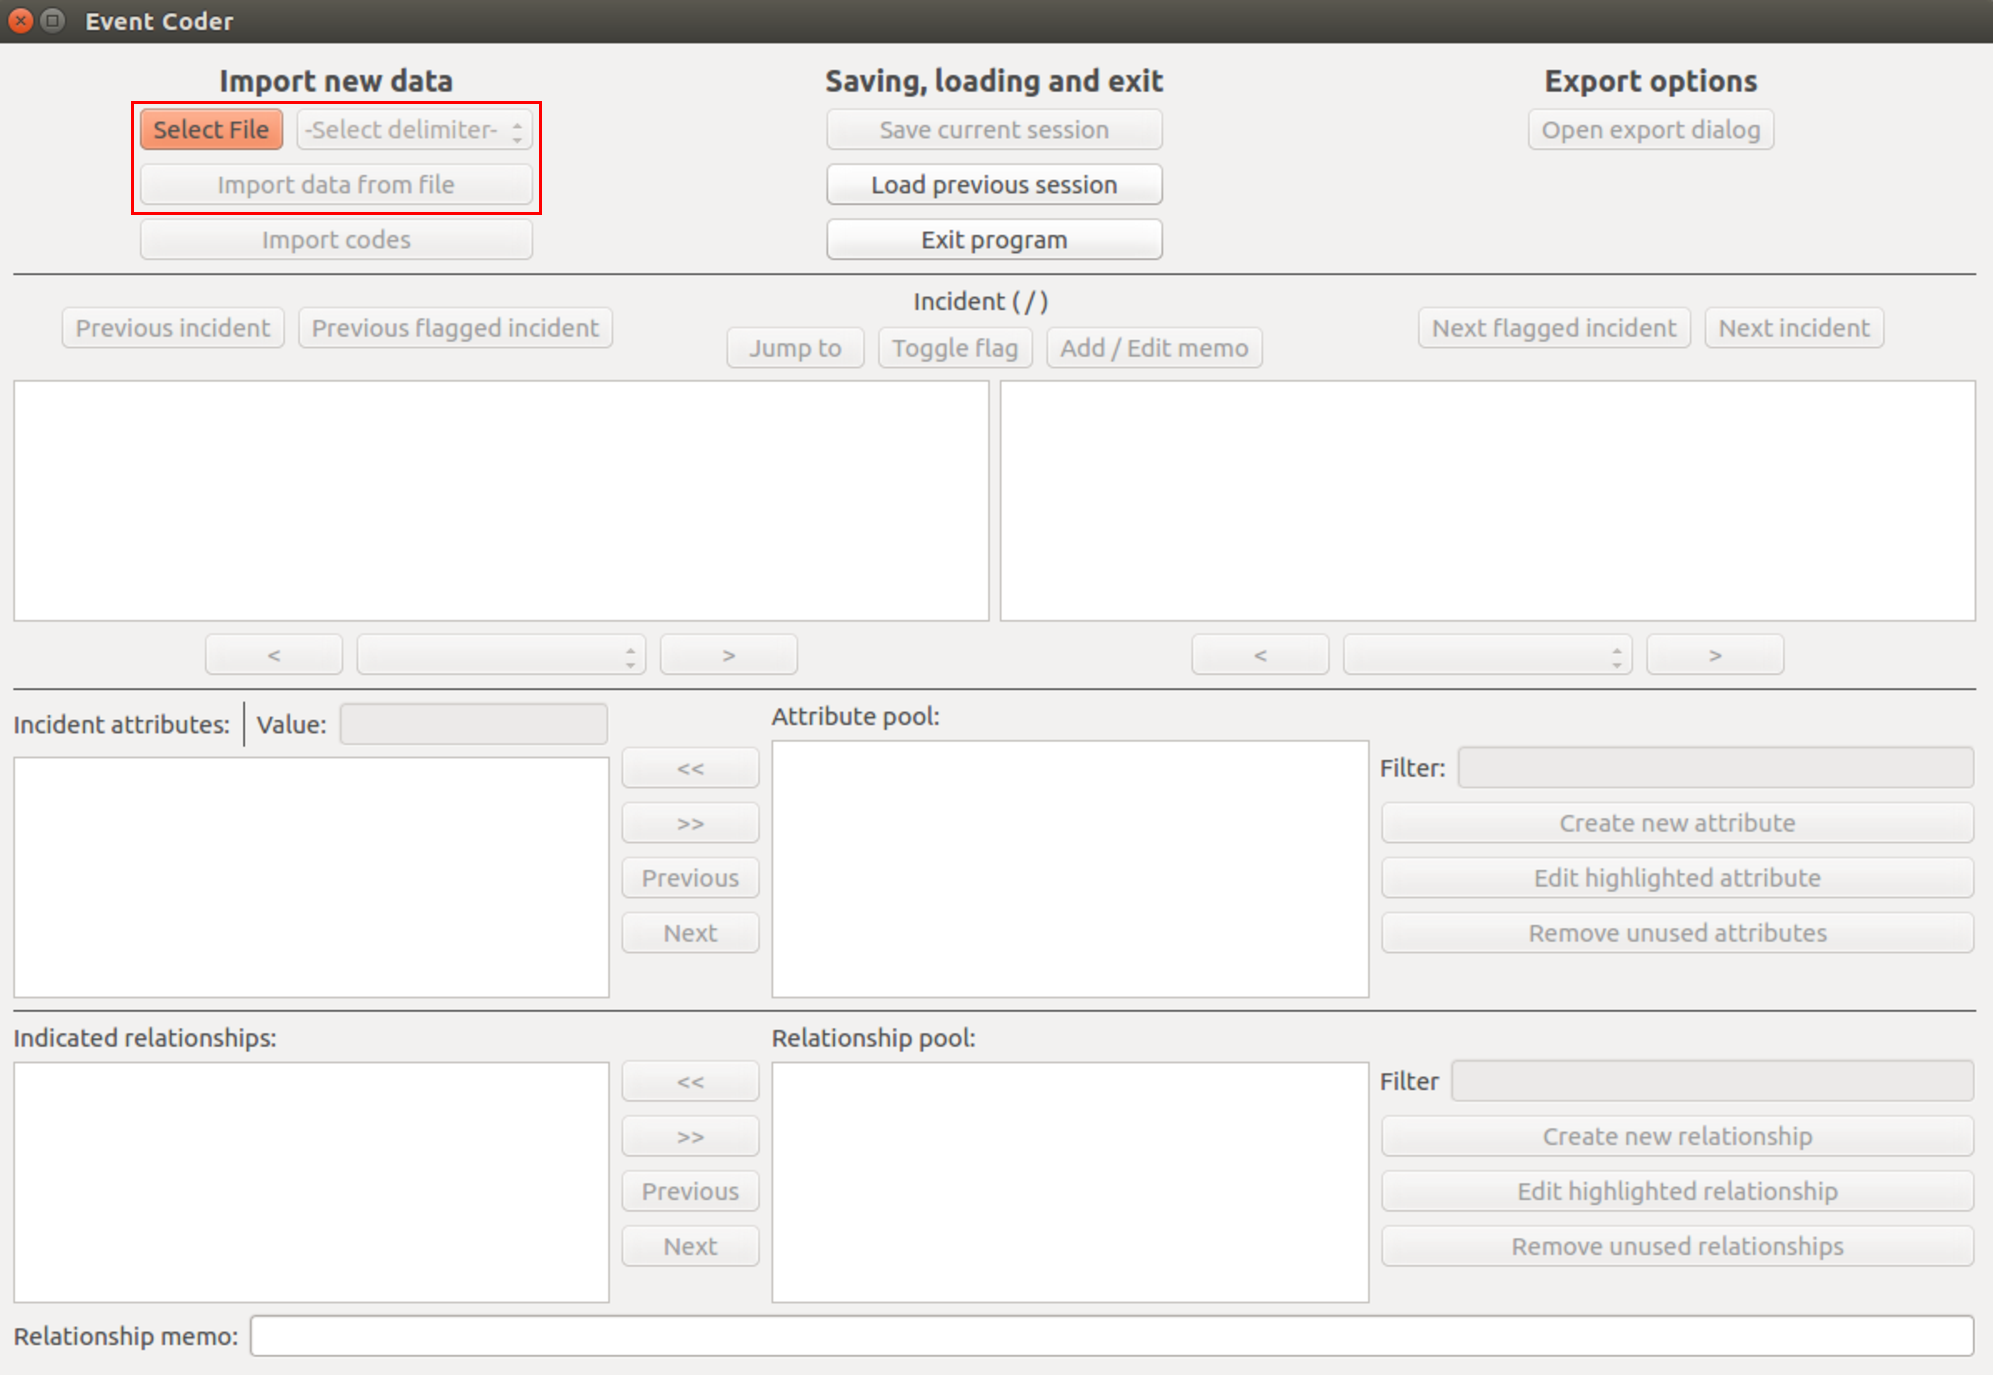
\includegraphics[width=100mm]{Screenshot_0.pdf}
  \label{fig:importoptions}
\end{figure}

\subsection{Problems when importing data}
\label{sec:importerrors}

If you (1) selected a valid csv-file, (2) selected the correct delimiter for this file, and (3) structured your data set using instructions offered in section \ref{sec:datasets}, you should encounter no problems when importing the data. If something goes wrong when importing data, then the problem will usually lie with one of these three points.

One possibility is that you have not selected a valid csv-file. I have encountered a few people that have tried to create csv-files from (for example) xls-files by simply changing the file extension. Doing this will not actually create a valid csv-file that can be read by the program. The correct way for creating csv-files is to use the \textbf{Save as} option in your spreadsheet editor, and select to save the file with the \textbf{*.csv} extension.

If you selected the wrong delimiter, the program will usually import the data, but it will fail to distinguish between different columns of the data set, and possibly assume that the entire dataset only contains one column. This should be obvious from the texts displayed by the program. In this case, simply import the data again, using the correct delimiter. 

If you see the error message displayed in figure \ref{fig:importerror}, this means that some cells of your data set probably contain newline symbols and/or carriage return symbols that need to be removed before importing data (see section \ref{sec:othernotesdatasets}).

\begin{figure}[h!]
  \centering
  \caption{Data import error report.}
  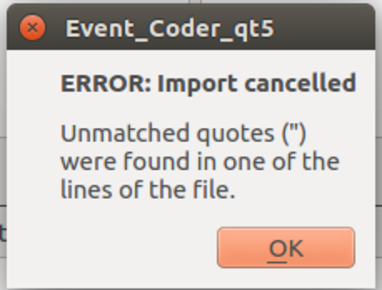
\includegraphics[width=40mm]{Screenshot_1.pdf}
  \label{fig:importerror}
\end{figure}

If you are certain that you made no mistakes in one of these points, and you still encounter problems when importing your data set, then you may have encountered a bug in the program that needs to be fixed. In that case, please get in touch with me (see chapter \ref{chap:contactdetails}).

\section{Saving and loading data}
\label{sec:savingloadingdata}

Coding a data set typically will take a long time, which is why the program allows you to save your progress, and to load the saved session at another moment. Saving data can be done by clicking the \textbf{Save current session} button (see figure \ref{fig:saveload}). A file dialog will appear, asking you to select a location to store the file, as well as a name for the file. The files will always be saved with the ``.sav'' extension.

If you want to load a previously stored session, click the \textbf{Load previous session} button (see figure \ref{fig:saveload}). A file dialog will appear, allowing you to navigate to, and select the file that you wish to load. 

\begin{figure}[h!]
  \centering
  \caption{Saving and loading files.}
  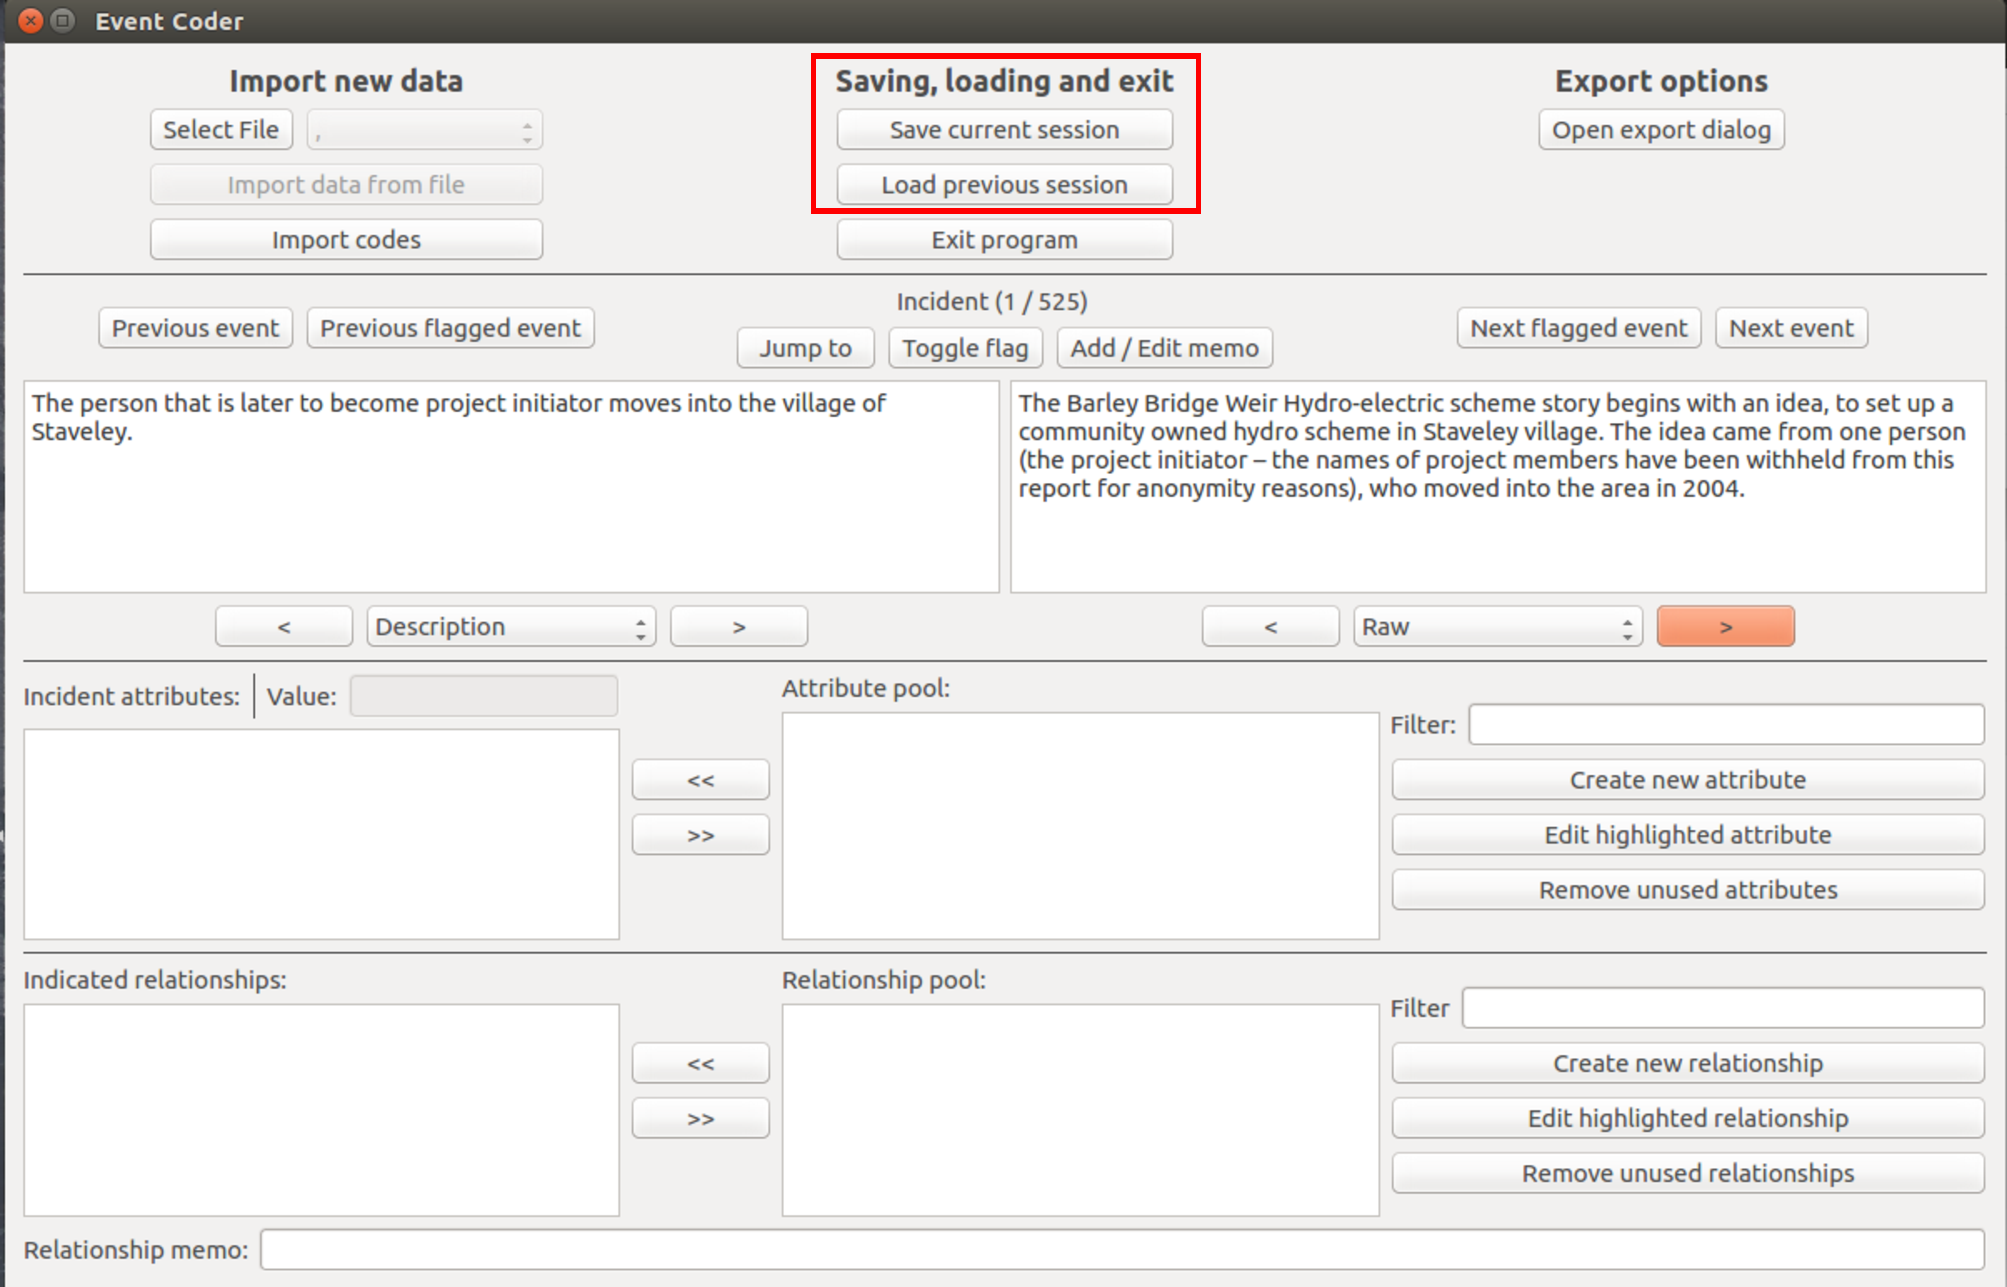
\includegraphics[width=100mm]{Screenshot_2.pdf}
  \label{fig:saveload}
\end{figure}

\section{Importing existing codes}
\label{sec:importingcodes}

Coding data is typically an iterative process, and it is possible that, during the coding process, the user makes changes to the data set being coded, for example, by adding new rows of data, by adding new columns of data, or by changing the contents of data cells. The program therefore allows the user to import existing codes from an old version of a given data set into a new version of the same data set. 

\begin{figure}[h!]
  \centering
  \caption{Importing codes.}
  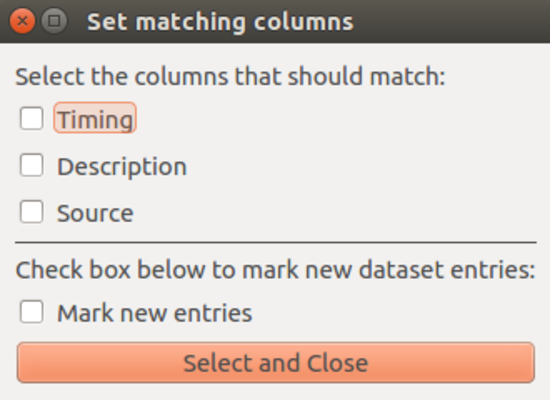
\includegraphics[width=100mm]{Screenshot_3.pdf}
  \label{fig:importcodesfig}
\end{figure}

The procedure for importing codes involves the following steps:
\begin{enumerate}
\item{The user should first make sure that the codes assigned to the \textbf{old version} of the data set are stored, by using the \textbf{Save session option} (see section \ref{sec:savingloadingdata}). At a later step, we will import the codes from this save file. For this example, we refer to this files as \textbf{Saved\textunderscore Codes.sav}.}
\item{After saving the codes assigned to the \textbf{old version} of the data set, we can import the \textbf{new version} of the data set, using the procedure described in section \ref{sec:loadingnewdataset}. Thus, the steps taken here are the same as when you would start coding a completely new data set.}
\item{After the \textbf{new version} of the dataset has been loaded, you should click the \textbf{Import codes} button (see figure \ref{fig:importcodesfig}). You will first be shown a warning dialog, just to make sure that you can double check what you are doing. If you select \textbf{Ok} in the warning dialog, you will be shown a file dialog. Use this dialog to find the file with your saved codes (\textbf{Saved\textunderscore Codes.sav} in this example). Select and open this file.}
\item{A new dialog will appear, the specific contents of which will depend on the contents of your data sets. An example is shown in figure \ref{fig:importcodesfig}, but yours will probably look different. The dialog will show the columns that the old version of your data set and the new version of your data set have in common. Here, you need to select those columns that the program can use to match entries in the \textbf{old version} of the data set with entries in the \textbf{new version} of the data set. The program will look at the data in the selected columns of both files. If it finds a row of data in the \textbf{new version} of the data set and a row of data in the \textbf{old version} of the data set that have the exact same contents in the selected columns, then the program will decide that these rows of data are the same. The program will then ensure that all the codes that are somehow associated with the row of data in the \textbf{old version} of the data set, are also associated with the corresponding row of data in the \textbf{new version} of the data set. For this to work correctly, the rows of data in both data sets need to be unique. For example, if you select only one column, which has the same contents in multiple rows in one or both of the data sets, then the program will not be able to decide which codes are associated with which row of data. \textbf{In this case the codes will probably be assigned to the new data set erroneously, without warning!\footnote{In a later version of the program I will attempt to prevent this from happening altogether.} It is therefore very important that you always select a combination of columns that allows the program to identify each row of data individually.} Usually, it should be enough to select the column that indicates the timing of the incident, and the column that describes what happened in that incident, because having two incidents with the exact same timing, and the exact same contents (description) would probably never make sense, because they would describe the same (inter)action, making one of them redundant. See figure \ref{fig:importingcodesdiagram} for a schematic overview that may help to understand the process.}
\item{You also have the option to have the program mark any new entries in the \textbf{new version} of the data set. This means that, while checking the columns you have selected, the program will also remember any rows of data in the \textbf{new version} of the data set that it could not match to any rows of data in the \textbf{old version} of the data set. These entries will be marked (see \ref{sec:markingincidents}), so that you can easily find them while coding the data.}
\item{If you happened to have changed data in one of the rows of the data set, that is, the row was already present in the \textbf{old version} of the data set, but you changed some of the contents of that row of data in the \textbf{new version} of the data set (in one of the selected columns), that row of data will be treated as new entry, and any codes assigned to that entry will be lost.}
\item{The program should now return to the main screen, and any attribute codes and relationship codes that were present in the save file that you loaded should now also be available in the current session. Moreover, any incidents that already had codes assigned to them in that save file should now also have those codes assigned to them in the current session.}
\end{enumerate}

\begin{figure}[h!]
  \centering
  \caption{Schematic overview of matching of data set entries.}
  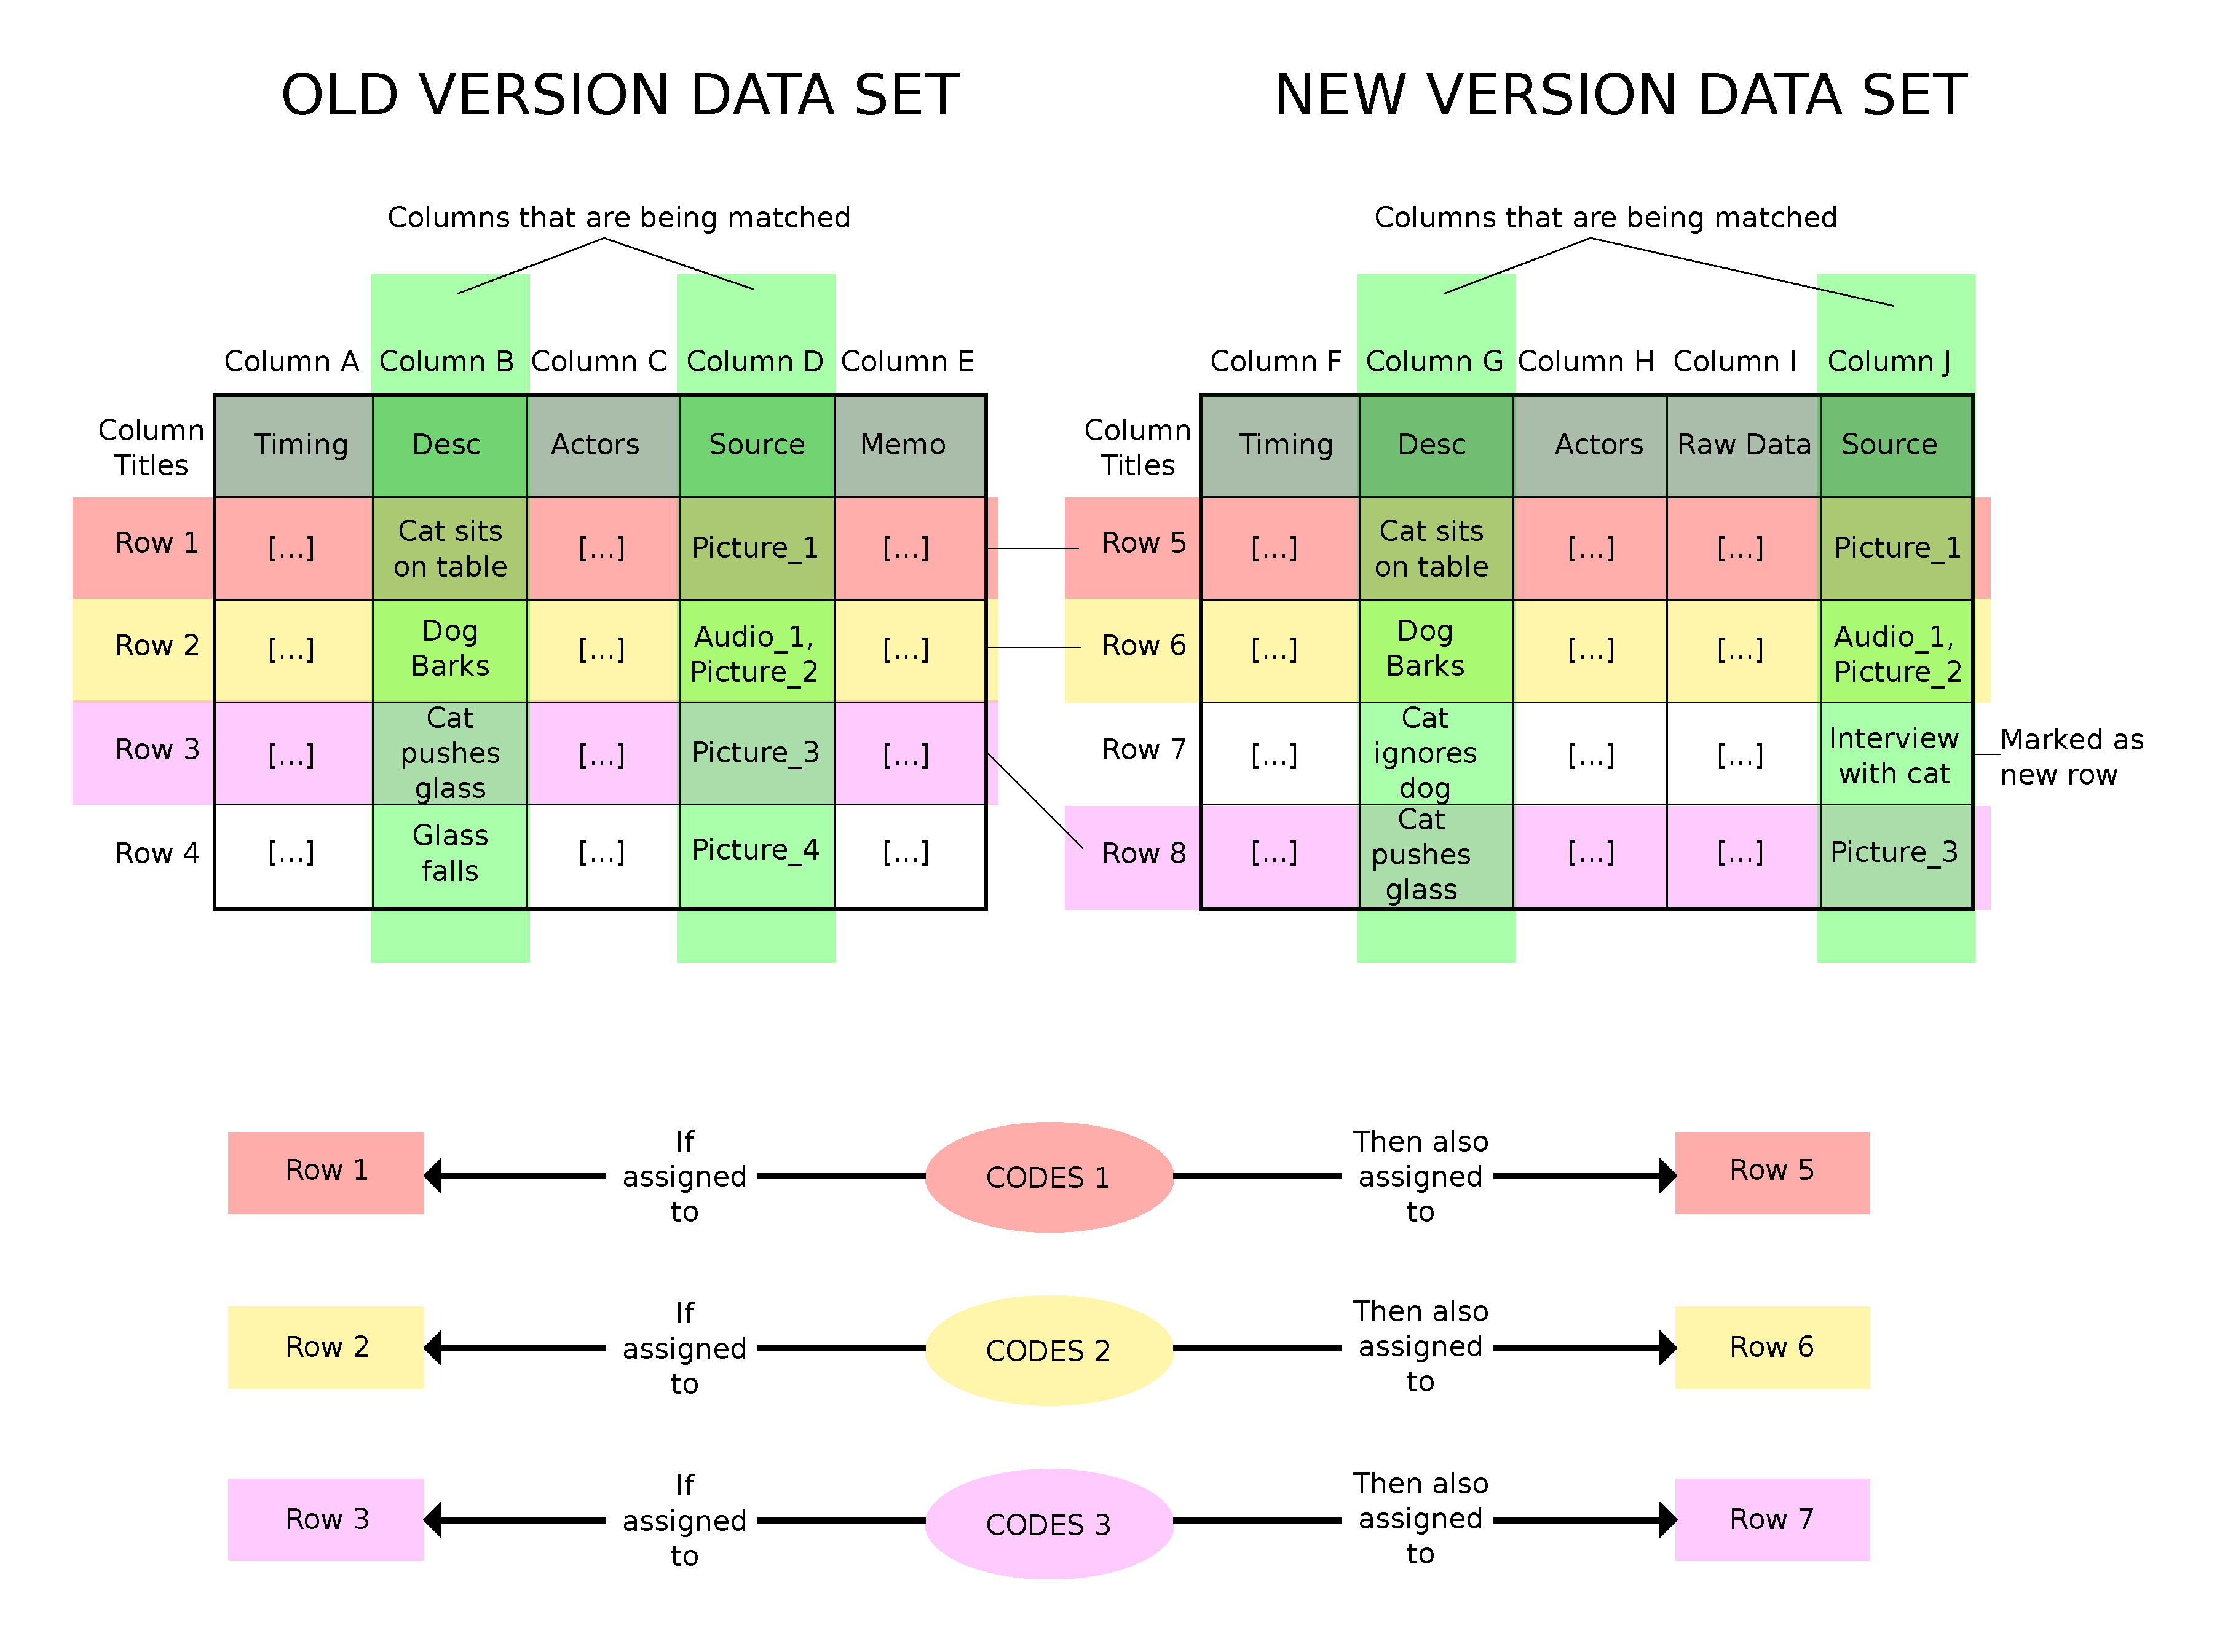
\includegraphics[width=100mm]{Diagram_1.pdf}
  \label{fig:importingcodesdiagram}
\end{figure}

\subsection{Problems when importing codes}
\label{sec:problemsimportingcodes}

There are several things that could go wrong when importing codes from an old data set into a new one. One problem would occur if you do not select any columns to be imported in the appropriate dialog. In this case the program will simply report that no columns were selected, and take no further action. Another similar problem would occur if you try to import codes from a data set that has now columns in common with the data set that is loaded into your current session. In this case the dialog where columns can be selected will be empty (except for the option to mark new entries). If you try to proceed, the program will behave as if no columns were selected (see above), report an error, and take no further action.

Another problem may be that some of the codes assigned to entries in the \textbf{old version} of the data set do not get imported into the \textbf{new version} of the data set, even though these entries appear in both. This should only happen if something changed in the contents of these entries (and only in the contents of those columns that the program tries to match). Even if you made only small changes in the contents of the selected columns, the program will treat the corresponding entry as a new, uncoded entry. 

A more difficult problem will occur if you do not select columns that allow the program to identify each row of data in the \textbf{old version} and/or the \textbf{new version} of your data set individually (see the box below for an explanation).

\begin{framed}
  \textbf{Example to illustrate problem when importing non-unique rows}

  First, imagine that you select two columns (\(C_1\) and \(C_2\)), the contents of which need to be matched by the program. Second, imagine that in the \textbf{old version} of the data set, there exist two incidents (two rows in the data set; \(I^{old}_1\) and \(I^{old}_2\)) that have identical data in those columns. In addition, imagine that the sets of codes (\(S_1\) and \(S_2\)) that you assigned to these two incidents are different (\(S_1 \rightarrow I^{old}_1\) and \(S_2 \rightarrow I^{old}_2\)).

  When comparing the two versions of the data set, the program encounters one of these rows of data \(I^{old}_1\). If it also encounters a row of data in the \textbf{new version} of the data set that has the exact same data in \(C_1\) and \(C_2\) (let us call this row \(I^{new}_x\)), it will think it has found a match, and assign the corresponding codes to the corresponding entry in the \textbf{new version} of the data set (\(S_1 \rightarrow I^{old}_1\) becomes \(S_1 \rightarrow I^{new}_x\)). However, the program then proceeds, and it will also encounter the other row of data \(I^{old}_2\), the contents of which (in columns \(C_1\) and \(C_2\)) also match with those of \(I^{new}_x\). As a result, the program will simply overwrite the codes that already existed (\(S_1 \rightarrow I^{new}_x\) gets overwritten by \(S_2 \rightarrow I^{new}_x\)). More importantly, the program will not recognise that something has gone wrong, so it will do this work silently, without reporting any error (also see figure \ref{fig:overwritingcodes}).
\end{framed}

\begin{figure}[h!]
  \centering
  \caption{Codes that are silently overwritten due to multiple matches.}
  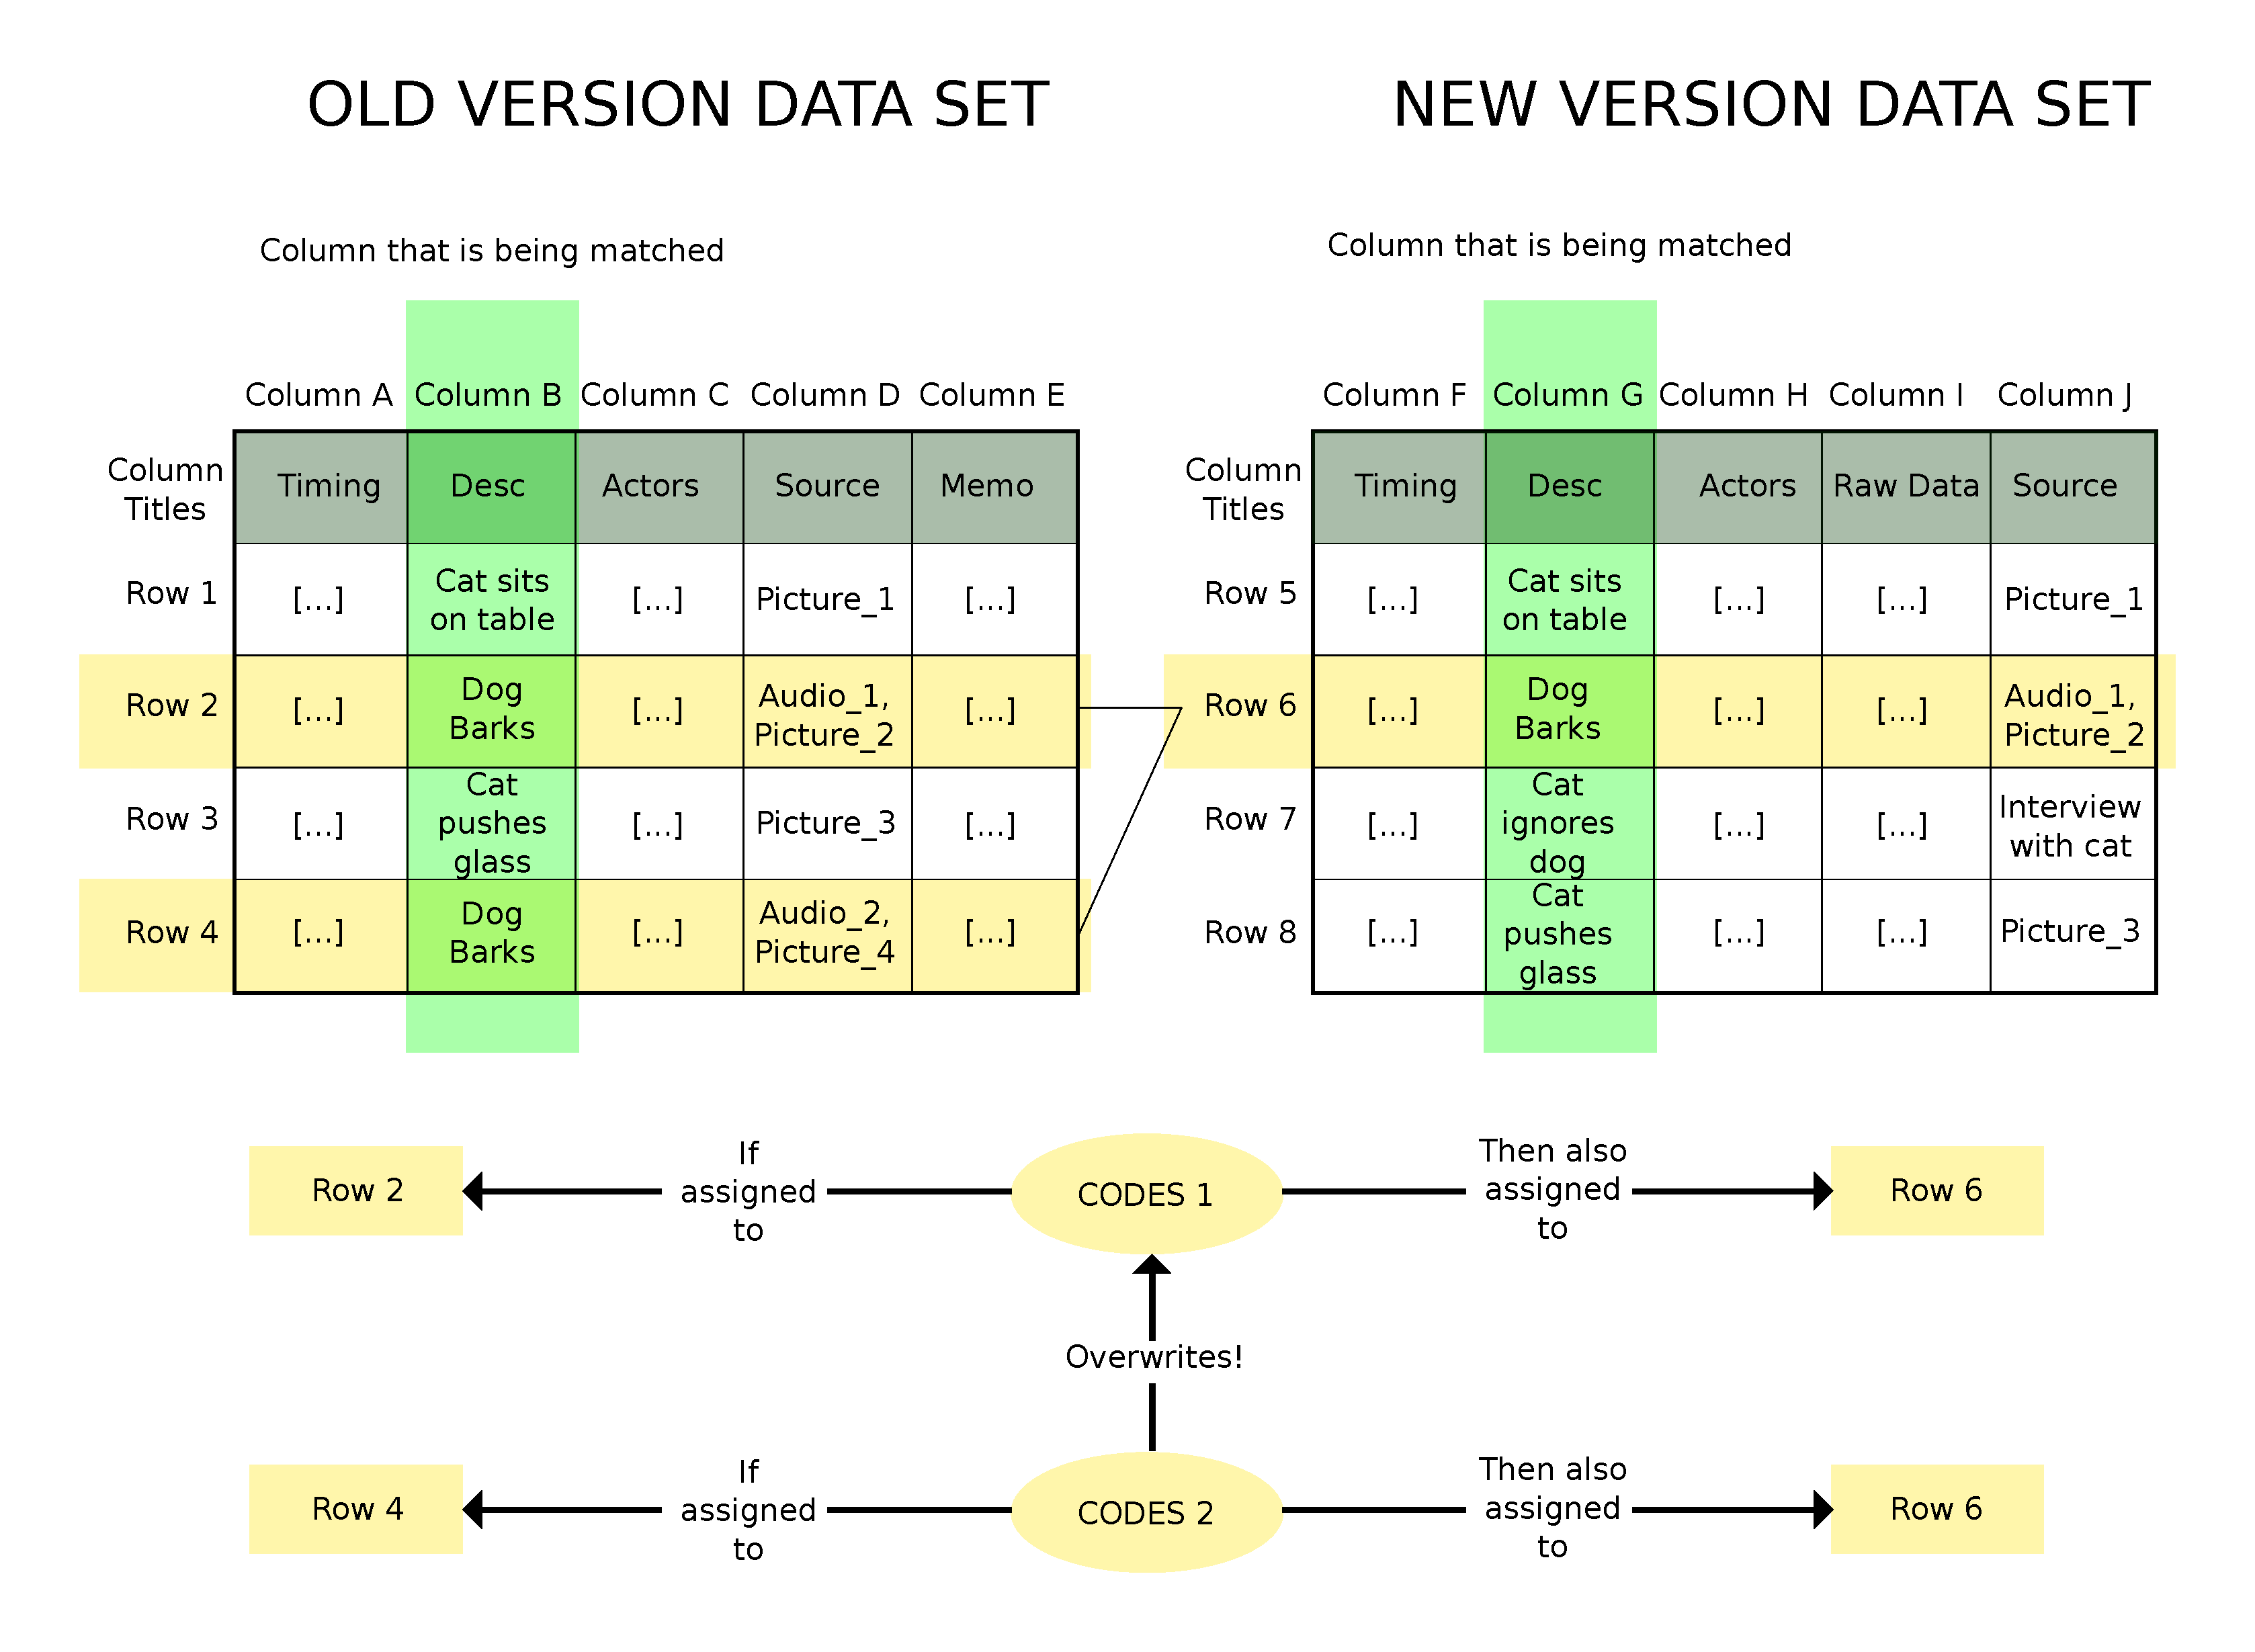
\includegraphics[width=100mm]{Diagram_2.pdf}
  \label{fig:overwritingcodes}
\end{figure}

To prevent this problem from occurring, you must always make sure that, based on the columns that you selected in the import dialog, the program will never find two rows of data that are exactly the same. As explained in section \ref{sec:importingcodes}, it should typically be enough to select (1) a column that indicates the timing of the incident, and (2) a column that contains the qualitative description of the incident itself (see section \ref{sec:datasets} for the assumptions that the program makes about how your data set is structured). It is unlikely that two incidents have the exact same contents in these two columns (because then they would simply refer to the exact same incident).

\section{Navigating through the data}
\label{sec:navigatingdata}

The program, to some extent, enforces a specific way to walk through your data set. As explained in section \ref{sec:datasets}, the program assumes that your data are chronologically ordered, with the incidents that occurred earliest at the top, and the incidents that occurred latest at the bottom. When you start coding a new data set, the program will always assume that you wish to start the coding process with the earliest incident. The program will present to you one incident at a time, showing you details on the currently selected incident in up to two fields (see figure \ref{fig:incidentsoverview}). 

\begin{figure}[h!]
  \centering
  \caption{Overview of incident navigation section.}
  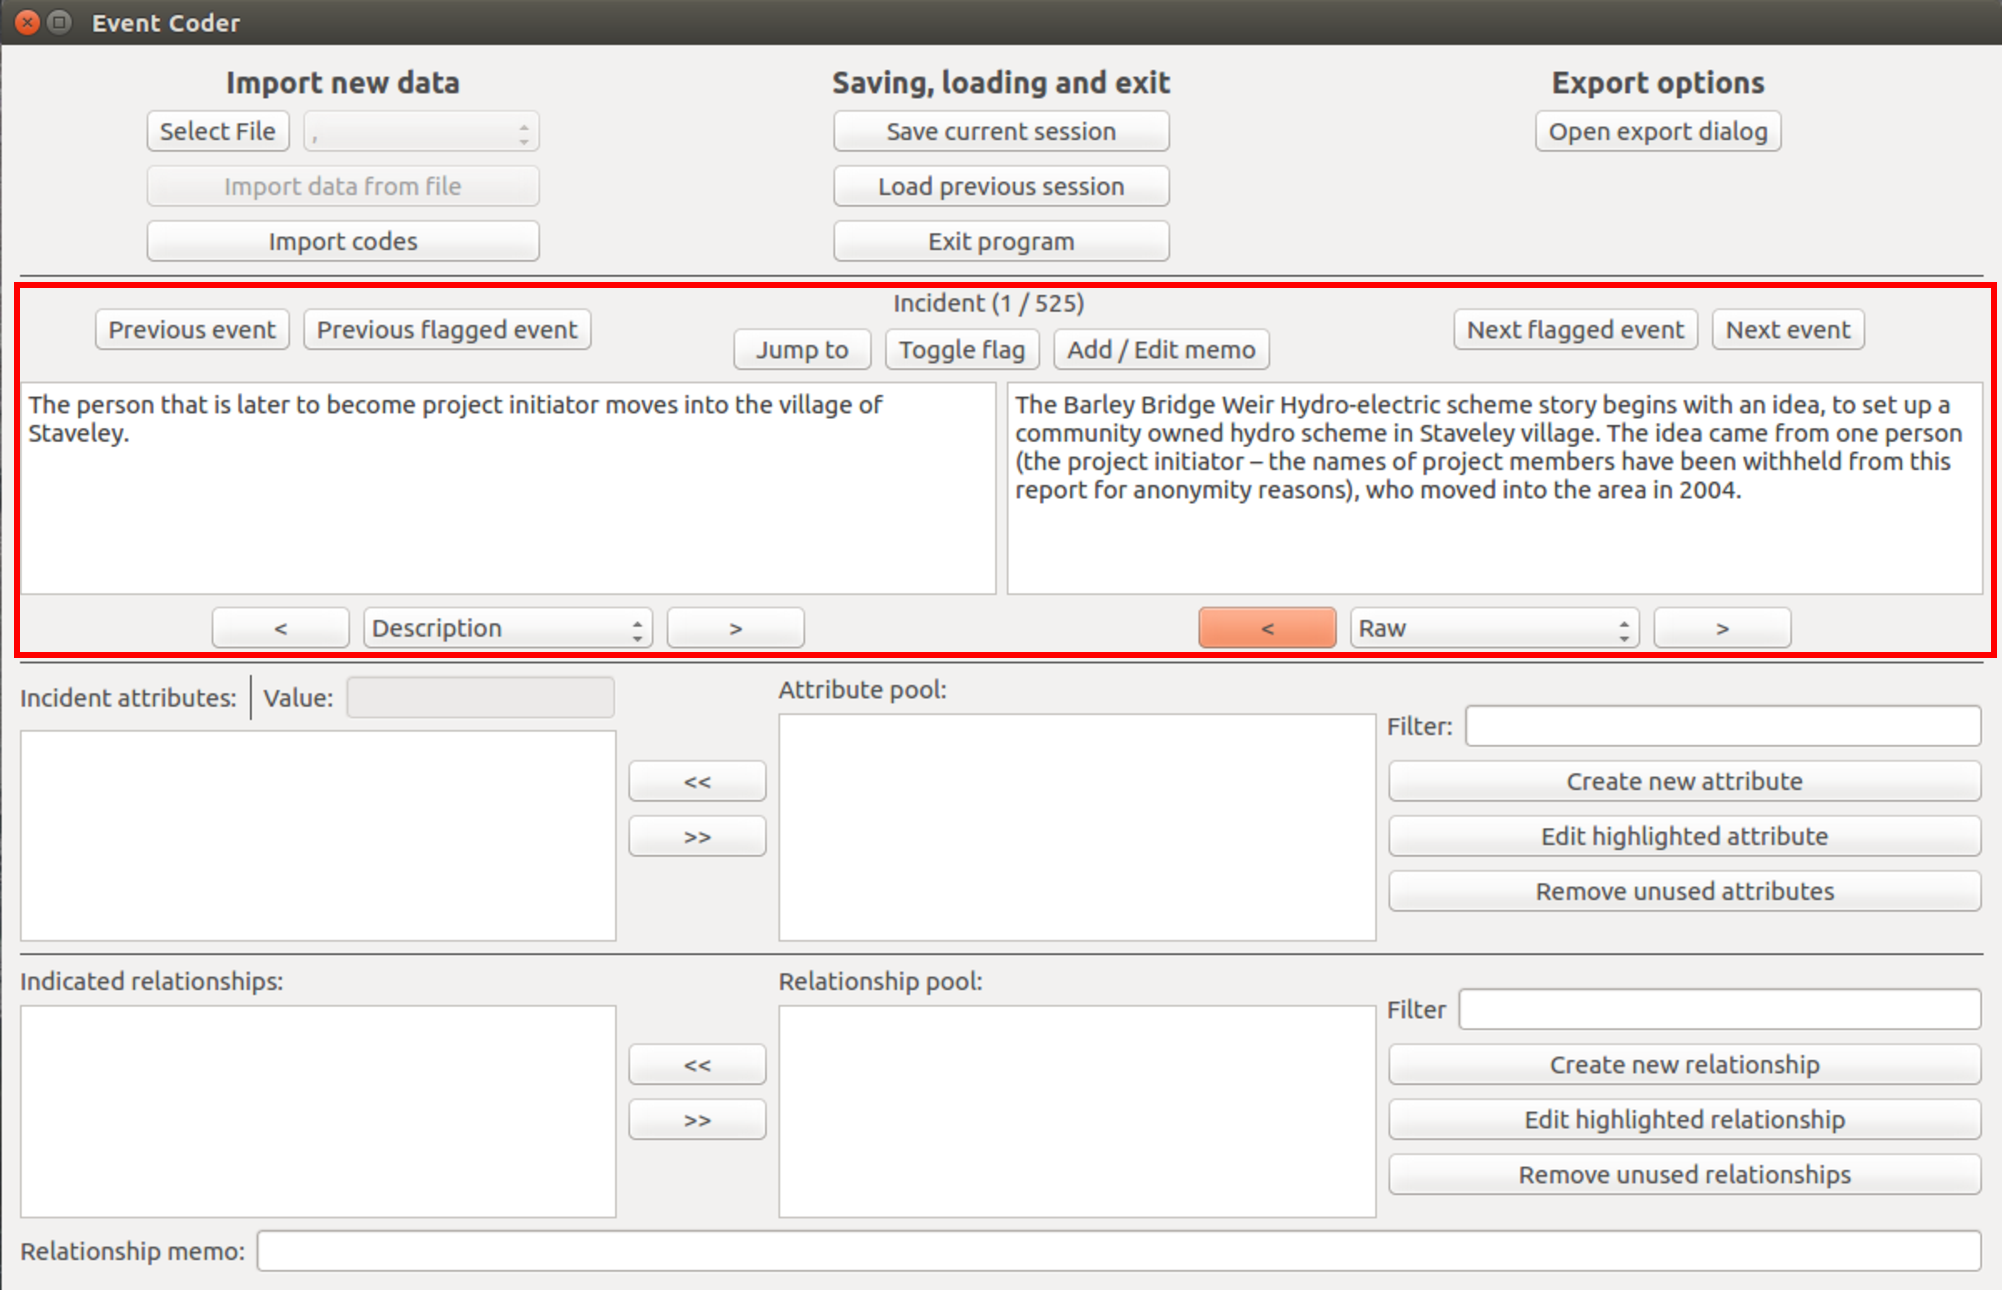
\includegraphics[width=100mm]{Screenshot_4.pdf}
  \label{fig:incidentsoverview}
\end{figure}

In the two fields, the program can display the contents of any of the columns of your original data set. Below each field, you will find buttons that you can use to choose which column of the original data set to display in the field (the first column of data is selected by default for both fields). The arrow buttons will go to the previous or next column, and the drop-down menu can be used to simply jump to a specific column. 

Typically, you will want to assign codes to the incidents based on the information provided in one or more columns of data, such as the description of the (inter)action that the incident captures, and possibly the raw text (from the sources of data) on which this description is based. The program can show up to two columns of data, which, in my own experience, is a nice balance between having a good overview, and not having to process too much information at a time.

Typically, you will create new codes on the fly (see chapter \ref{chap:usingtheprogram2}), assign appropriate codes to the current incident, and then move on to the next incident. Above the fields with the information on the current incident, you will see an indicator of which incident is currently selected (``\textbf{Incident ([current]/[total])}''). To navigate the incidents, use the buttons above the fields with the texts (see figure \ref{fig:incidentsoverview}). These buttons are pretty straightforward. The \textbf{Previous incident} button navigates to the previous incident in the data set. If the currently selected incident is the first in the data set, clicking this button will let you jump to the last incident in the data set. The \textbf{Next incident} button lets you navigate to the next incident in the data set. If the currently selected incident is the last incident in the data set, clicking this button will let you jump to the first incident in the data set.

You will also see a button called \textbf{Jump to}. Clicking this button will open a small dialog that allows you to type the index number of the incident that you want to jump to. If you type an 'illegal' number (e.g., a number below 1, or a number that exceeds that total number of incidents in the data set) nothing will happen. 

\subsection{Marking incidents}
\label{sec:markingincidents}

In the area demarcated in figure \ref{fig:incidentsoverview}, you will also find three buttons that refer to flagged incidents (\textbf{Previous flagged incident}, \textbf{Next flagged incident}, and \textbf{Toggle flag}). Flags can be used to mark incidents that you would like to return to later. If you click the \textbf{Toggle flag} button, an exclamation mark will appear next to the index to show that this incident is currently flagged (see figure \ref{fig:flaggedincident}).

\begin{figure}[h!]
  \centering
  \caption{Indication of flagged incident.}
  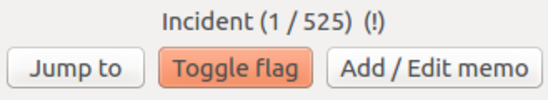
\includegraphics[width=40mm]{Screenshot_5.pdf}
  \label{fig:flaggedincident}
\end{figure}

If you later want to return to your flagged incident, you can use the \textbf{Previous flagged incident} or the \textbf{Next flagged incident} button. These buttons work similar to the \textbf{Previous incident} and the \textbf{Next incident} buttons, but they will skip all incidents that are not flagged. This should allow you to relatively easily find incidents that you flagged earlier.

\begin{framed}
\textbf{Automatically flagging new incidents when importing codes}
  
  As described in section \ref{sec:importingcodes}, when you import codes from a previously stored session into a new version of a data set, you will also have the option to mark any new incidents. This means that the program will automatically flag all incidents that are in the \textbf{new version} of the data set that you are currently coding, but that were not in the \textbf{old version} of the data set from which you are importing the codes. This allows you to always easily find the incidents that have not received any codes before. 
\end{framed}

\subsection{Adding memos to incidents}
\label{sec:memosincidents}

In any coding process it usually helps to write down your thoughts while coding, so that other people can, for example, read your motivations for assigning certain codes to a certain incident. Moreover, when coding larger data sets, you will often forget yourself why you made certain coding decisions. Typically, you would write down any relevant thoughts in the form of memos. The program allows you to associate memos with particular incidents. The memo associated with the current incident can be accessed by clicking the \textbf{Add / Edit memo} button. Clicking this button will open a small dialog, which consists out of a text field, where you can write your memo, and one button that allows you to save and close the memo dialog. If you want to add a memo, or edit an existing one, simply write the text you want to add, and then click the \textbf{Save and close} button. If you want to remove a memo you wrote earlier, simply delete all the text in that memo, and click the \textbf{Save and close} button. Each incident will have its own memo.

\section{Exporting data}
\label{sec:exportingdata}

In chapter \ref{chap:usingtheprogram2} I explain in depth how the coding program itself works. Once you have coded a data set, and you want to export the results, you can click the \textbf{Open export dialog} button. This will open a new dialog, where you can select several export options (see figure \ref{fig:exportdialog}).

\begin{figure}[h!]
  \centering
  \caption{The export dialog.}
  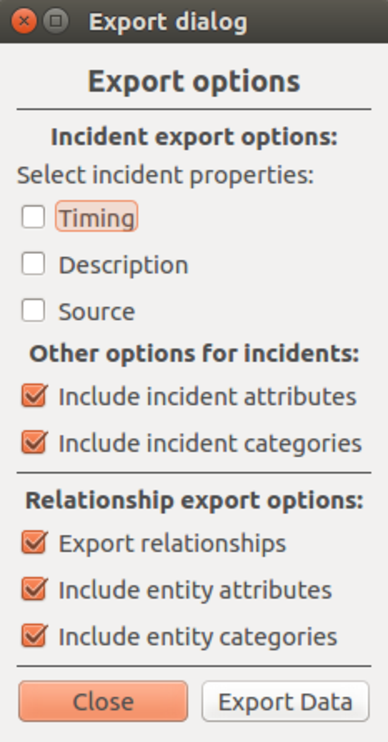
\includegraphics[width=100mm]{Screenshot_6.pdf}
  \label{fig:exportdialog}
\end{figure}

The first set of options, under the header \textbf{Incident export options}, allows you to assign properties to your incidents. These properties are simply the contents of the various columns of the data set that you imported. In fact, if you selected all the properties, using the corresponding tick boxes, one of the files exported will simply be a copy of the data set that you imported, with the only difference that every incident will be assigned a unique ID, numbered from 1 to \(N\), where \(N\) is the total number of incidents in your data set. These incidents, and any properties that you select form them, will be written to a file that is called \textbf{``Incidents\textunderscore Nodes.csv''}. As the name of the file suggests, this is a nodes file, which in this case is structured such that it can be immediately imported into Gephi, my favourite network visualisation program\footnote{See https://gephi.org. I offer no instructions on how to import data into Gephi here. Various guides for that are available elsewhere. Indeed, the data can also be imported into other software, although you might have to make small changes for that to work.}. Why it is useful to export the incidents and their properties in a node list will be clarified further below.

By default, the program will also export (1) all attributes that you have assigned to incidents, (2) all categories that you have assigned to incident attributes, (3) all relationships that you have assigned to incidents, (4) all attributes that you have assigned to entities in relationships, and (5) all categories that you have assigned to entity attributes. You can deselect any of these options, although categories can only be exported if their corresponding attributes are also exported. Depending on what options you select, the following will be exported:
\begin{enumerate}
\item{\emph{If you select to \textbf{Include incident attributes}, then three additional files will be created}: \textbf{``Incident\textunderscore Attributes\textunderscore Nodes.csv''}, a node list with the details (labels and descriptions) of all attributes that have been assigned to incidents, \textbf{"Incident\textunderscore Attributes\textunderscore to\textunderscore Incidents\textunderscore Edges.csv"}, an edge list that records which attributes have been assigned to which incidents (if values have been assigned, these will be recorded in the edge list as well), and \textbf{"Incident\textunderscore Attributes\textunderscore Matrix.csv"}, a matrix with incidents in the rows and attributes in the columns, showing a \(0\) in cells corresponding with incidents and attributes that are not associated, and showing a \(1\) in cells corresponding with incidents and attributes that have been associated. Alternatively, if a value has been assigned to an attribute, then that value will be reported in the cell, instead of a \(1\).}
\item{\emph{If you also select to \textbf{Include incident categories}, then two additional files will be created}: \textbf{"Incident\textunderscore Categories\textunderscore Nodes.csv"}, a node list with the details (labels and descriptions) of all categories that have been assigned to incident attributes, \textbf{"Incident\textunderscore Attributes\textunderscore to \textunderscore Categories\textunderscore \ Edges.csv"}, an edge list that records which incident attributes belong to which categories.}
\item{\emph{If you select to \textbf{Export relationships}, then five additional files will be created}: \textbf{"Relationships\textunderscore Nodes.csv"}, a node list with the details (labels and memos) of all relationships that have been assigned to incidents, \textbf{"Incidents\textunderscore to\textunderscore Relationships\textunderscore Edges.csv"}, an edge list that records which incidents are indicators for which relationships, \textbf{"Entities\textunderscore Nodes.csv"}, a node list with the details (labels and descriptions) of all entities that are in one or more relationships, \textbf{"Entities\textunderscore Edges.csv"}, and edge list that records which entities are in which type of relationship with each other, and \textbf{"Entities\textunderscore to \textunderscore Relationships \textunderscore Edges.csv"}, an edge list that records which entities are present in which relationships.}
\item{\emph{If you also select to \textbf{Include entity attributes}, then three additional files will be created}: \textbf{"Entity\textunderscore Attributes\textunderscore Nodes.csv"}, a node list with the details (labels and descriptions) of all attributes that have been assigned to entities, \textbf{"Entity\textunderscore Attributes\textunderscore to \textunderscore Entities\textunderscore Edges.csv"}, an edge list that records which attributes have been assigned to which entities (if values have been assigned, these will be recorded as well), and \textbf{"Entity\textunderscore Attributes\textunderscore Matrix.csv"}, a matrix with entities in the rows and attributes in the columns, showing a \(0\) in cells corresponding with entities and attributes that are not associated, and showing a \(1\) in cells corresponding with entities and attributes that have been associated. Alternatively, if a value has been assigned to an attribute, then that value will be reported in the cell, instead of a \(1\).}
\item{\emph{If you also select to \textbf{Include entity categories}, then two additional files will be created}: \textbf{"Entity\textunderscore Categories\textunderscore Nodes.csv"}, a node list with the details (labels and descriptions) of all categories that have been assigned to entity attributes, and \textbf{"Entity\textunderscore Attributes\textunderscore to\textunderscore Categories\textunderscore \ Edges.csv"}, an edge list that records which entity attributes belong to which categories.}
\end{enumerate}

Thus, in total, up to 16 files will thus be exported. These files will all be automatically saved in the \textbf{``export/''} folder, which can be found in the folder from which you run the program (if the folder was not already present, a new folder will be created). \textbf{Every time you export data, existing files in this folder will be overwritten.} Thus, if you want to keep old files, make sure that you copy them to another folder before exporting data again.

To understand more about what you could possibly do with all these files, please read chapter \ref{chap:whatisnext}.

\section{Log files and exiting the program}
\label{sec:logfilesandexiting}

It will probably come as no surprise to you that the default way to close the program is to click the \textbf{Exit program} button. Alternatively, you could close the dialog of the program in the same way you would close any dialog in your OS.

Just before the program closes, it will export a log file to the \textbf{"logs\"} folder that is located in the folder from which you run the program (if this folder does not exist yet, the program will create it). The log file will be time stamped with the date and time at which it was created. In the log file, you will find a lot of details of various operations that you have performed while using the program, such as navigating to other incidents, assigning or unassigning attributes and/or relationships to incidents, and several other things. These logs are created silently and automatically.

The logs are designed to help you make the coding process more transparent. For example, they may help you retrace your steps if at some point in the coding process you run into some kind of problem, and do not remember how you got there. The log also records which columns of your data set you were expecting when assigning certain attributes or relationships, helping you to remember on what information you based your decision to assign these codes. I do not expect that anyone will be terribly interested in every expecting these log files, but it may be reassuring to know that they are there if you need them.  


\chapter{Using the program: Coding features}
\label{chap:usingtheprogram2}

\section{Introduction to coding}
\label{sec:introductiontocoding}

Now we get to the core ``stuff'' of what the \textbf{\emph{Event Coder}} program is all about: Coding the data. In this program the coding options are divided into two main modules, \textbf{Attributes} and \textbf{Relationships}, which can be used in various ways, and which do not necessarily have to be used together. In this chapter, I will explain both coding modules in depth, and offer some basic suggestions for how they could be used.

\section{The Attribute module}
\label{sec:attributemodule}

We will first focus on the module that can be used to associate attributes with incidents. I decided to use the term attributes in this case, because these entities will generally be used to identify relevant properties of the incidents. Some example of different sorts of attributes that I thought of myself, are as follows:
\begin{itemize}
\item{\emph{\textbf{(Inter)action types}}: Given that incidents are assumed to capture (inter)actions (see section \ref{sec:datasets}), one thing we possibly want to do is to use attributes to identify different types of action. For example, imagine that we have a data set that captures interactions between cats and dogs. Examples of attributes that capture different types of such (inter)actions are \emph{barking}, \emph{meowing}, \emph{chasing cats}, \emph{hissing at dogs}, and so on. We would have a list of such attributes, each describing an individual type of (inter)action, and assign these to incidents where appropriate. The point here is to treat each individual incident is the occurrence of a particular type of (inter)action (see figure \ref{fig:usesofattributes}.A).}
\item{\emph{\textbf{Colligated events}}: On some occasions, the researcher using the program might not necessarily be interested in the (inter)actions described by his/her incidents per se, and he/she might instead be more interested in some more abstract event for which the incidents serve as indicators. For example, imagine someone who made a data set that records the interactions between two primitive clans that inhabit roughly the same geographical area. The incidents could in this case be empirical descriptions of the interactions that involve members from both clans. Some of these interactions may refer to occasions where members of the clans exchanged certain objects or services, which one might see as indicative of \emph{trading} between the clans. Other interactions may refer to occasions where members of the clans attack each other, which one might see as indicative of \emph{conflict} between the clans. One could of course assign such interaction types as attributes (see above), but one would thereby overlook that some of the exchanges (described by more than one incident) and some of the attacks (described by more than one incident) refer to the same instances of \emph{trading} or \emph{conflict}. The point here is thus to use attributes to indicate which incidents ``group'' together. We could, for example, distinguish between different instances of trading by numbering them (see figure \ref{fig:usesofattributes}.B). If desirable, we could even make explicit that the different versions of the same attribute (e.g., \emph{Trading\textunderscore 1} and \emph{Trading\textunderscore 2}) belong together by assigning a category called \emph{Trading} to them. Attribute categories are explained further on in this section.}
\item{\emph{\textbf{Value changes}}: There are approaches to studying social processes that treat each incident inherently as a change. In some cases, one could even want to use values to express by how much something changes. Imagine that you check how much money you currently have on your bank account, and you find (to your surprise) that you are in debt. In a flurry of irrational behaviour, you decide to reconstruct all your incomes and expenses in an event data set, to reconstruct how you got to this point (Maybe it works therapeutic? Who knows?). To capture your incomes and expenses, you could simply create two attributes: \emph{Money increase} and \emph{Money decrease}, and assign these to incidents in your data set accordingly. As will be explained further on in this section, you have the possibility to assign a value to any attribute that is also assigned to an incident. This value will always be unique to that particular ``incident-attribute pair''. This allows you to track, over time, how much money went in or out (although values do not necessarily have to be numerical), and by how much (see figure \ref{fig:usesofattributes}.B).}
\end{itemize}

\begin{figure}[h!]
  \centering
  \caption{Three possible uses of attributes.}
  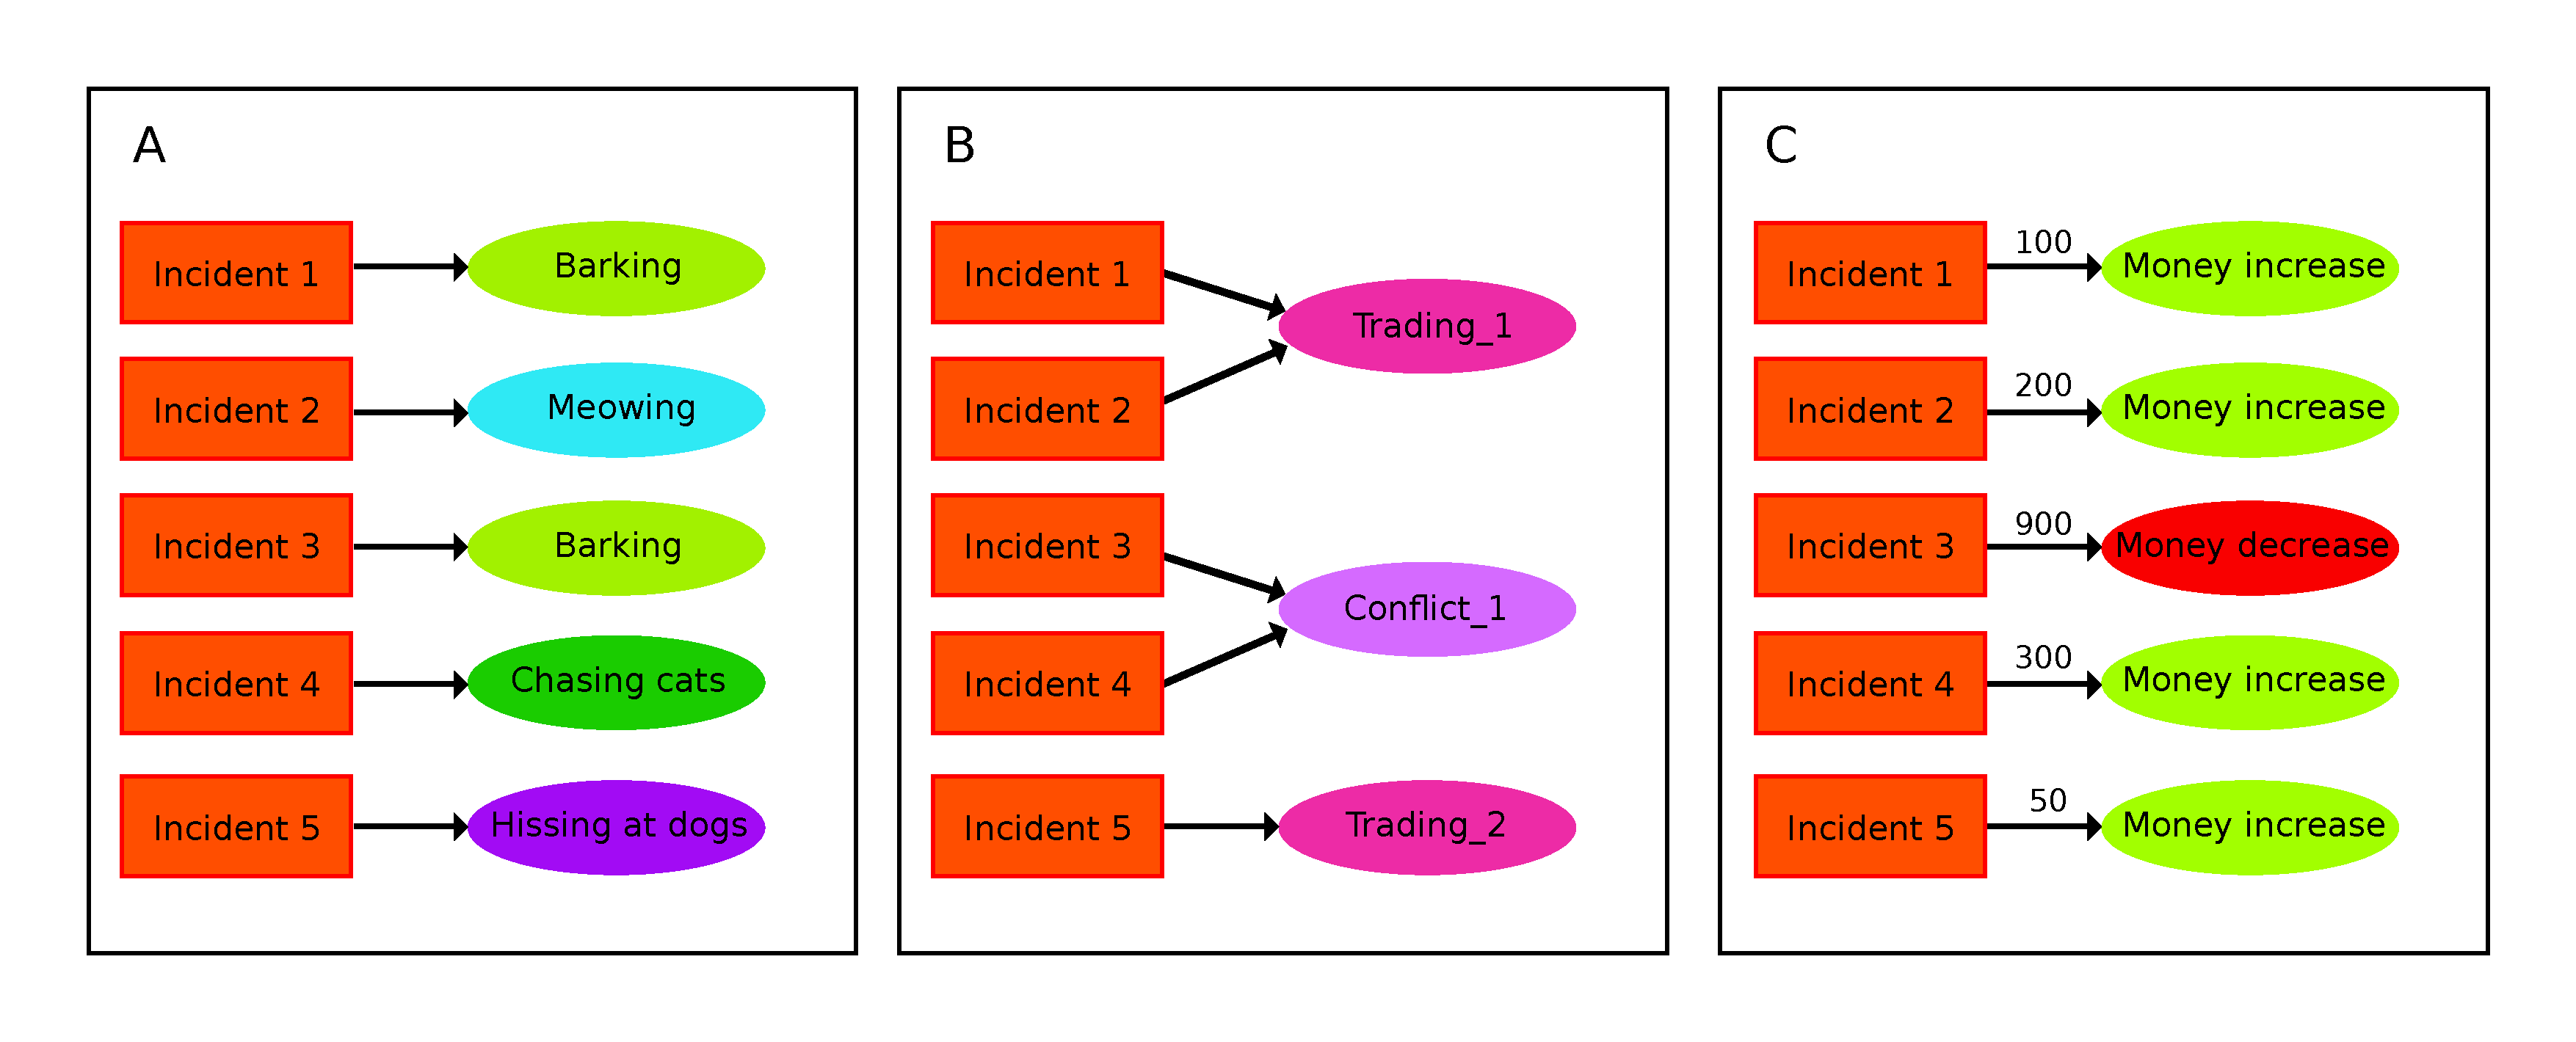
\includegraphics[width=100mm]{Diagram_3.pdf}
  \label{fig:usesofattributes}
\end{figure}

Of course, other uses of attributes are thinkable. One could for example also use attributes to identify the actors that are involved in the activities described in incidents, or to identify the places where the activities described in the incident take place (but also see section \ref{sec:relationshipmodule} for an alternative approach to coding for this). I tried to design this module in a way that accommodates different approaches. In reality there are no great technical differences in the way that attributes are associated with incidents in the three different scenarios visualised in figure \ref{fig:usesofattributes}. What the program does, in the background, is always more or less the same. Taking different approaches to using attributes is therefore primarily a matter of how the user thinks about them, and how this thinking fits in the overall research design of the user. Of course, the possibilities are not limitless. A lot will depend on how you are actually able to use the attributes after you export them. To read more details about this, please see section \ref{sec:exportingdata} and chapter \ref{chap:whatisnext}.

\subsection{Creating new attributes}
\label{sec:creatingnewattributes}

If you have just started a new session, then the attributes module will look more or less as illustrated in figure \ref{fig:attributemodule}.

\begin{figure}[h!]
  \centering
  \caption{The attribute module.}
  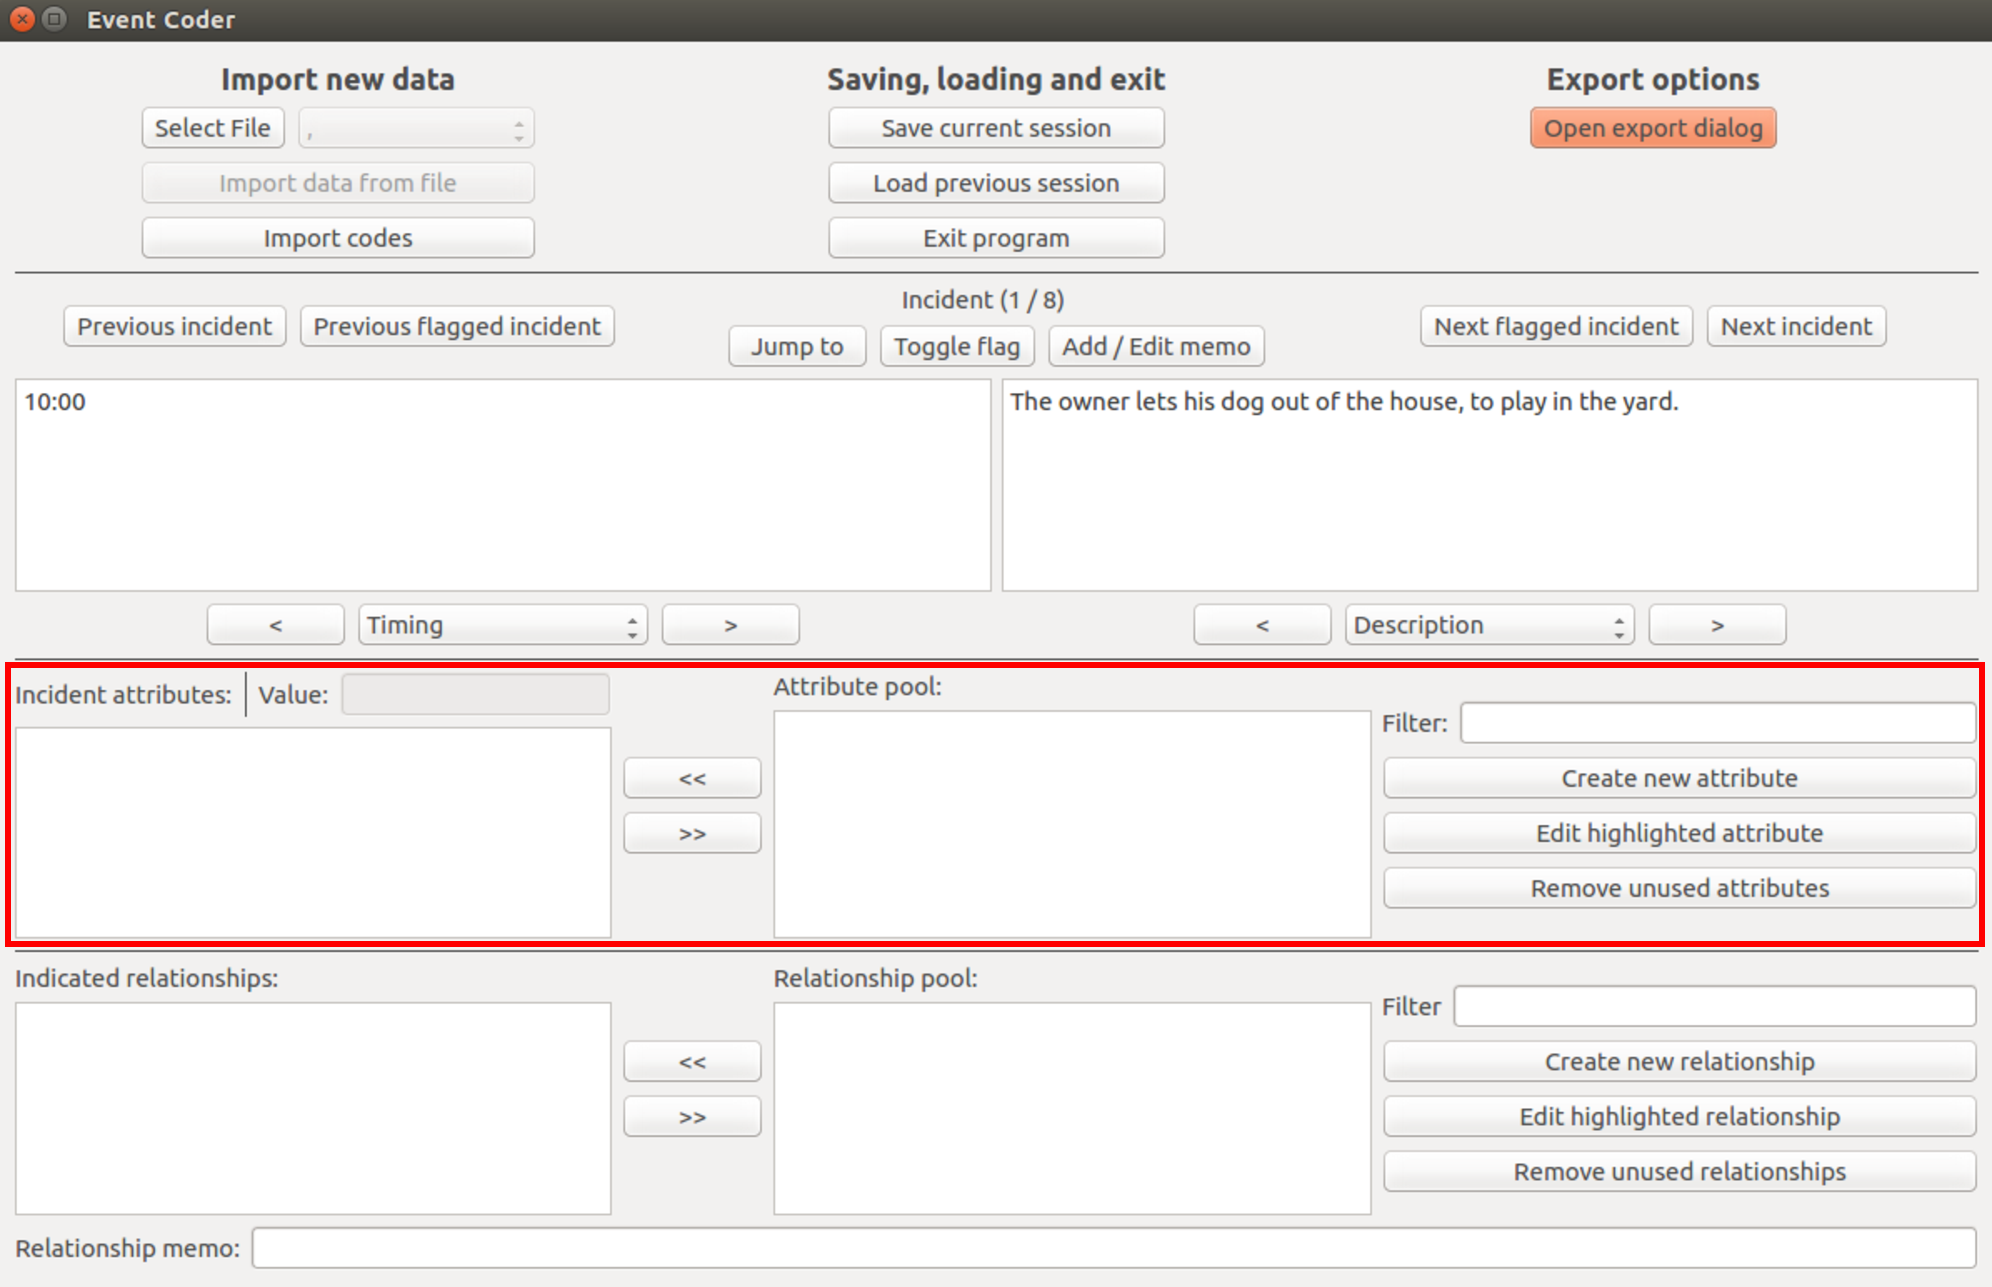
\includegraphics[width=100mm]{Screenshot_7.pdf}
  \label{fig:attributemodule}
\end{figure}

No attributes have been created yet, so the list of (assigned) \textbf{Incident attributes} (left) and the (unassigned) \textbf{Attribute pool} (right) will be empty. As I will explain in more detail below, attributes that are assigned to the incident will always appear in the left field. The ``pool'' of attributes from which one may select attributes to assign is shown in the right field.

If you wish to assign attributes, you will first need to create them. For this, you have to click the \textbf{Create new attribute button} on the right side of the module (see figure \ref{fig:attributemodule}). This will open a new dialog, which looks like the one shown in figure \ref{fig:attributedialog}.

\begin{figure}[h!]
  \centering
  \caption{The attribute dialog.}
  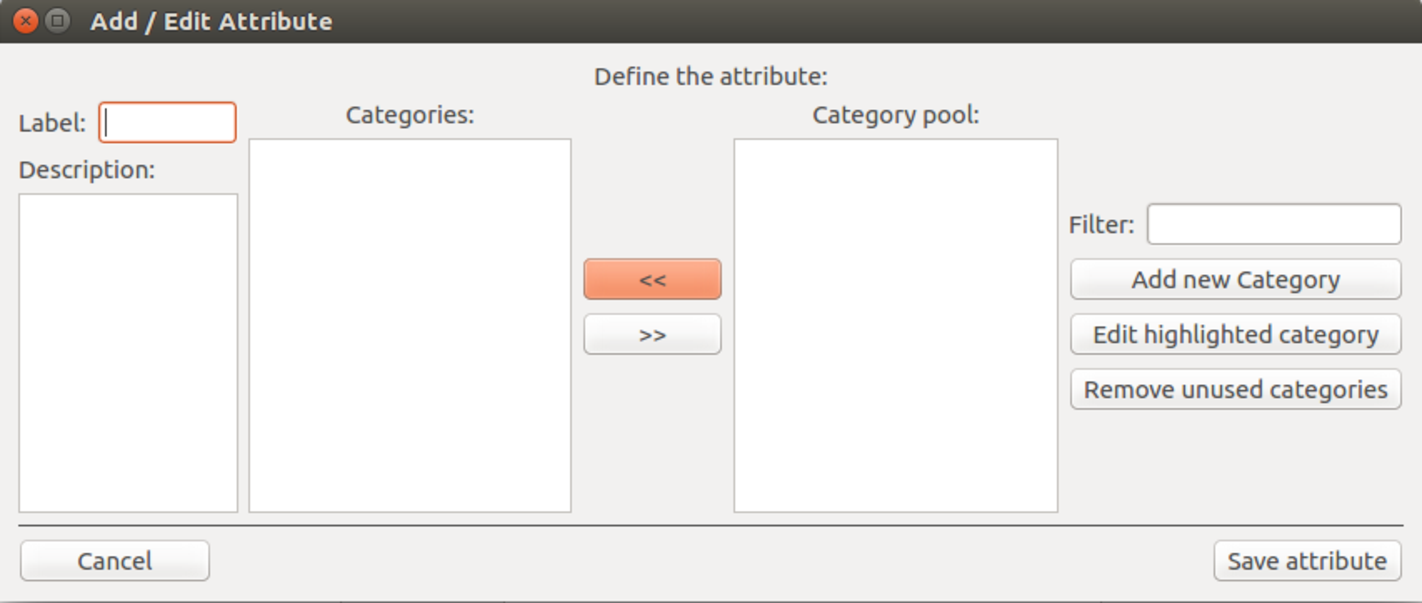
\includegraphics[width=100mm]{Screenshot_8.pdf}
  \label{fig:attributedialog}
\end{figure}

If you want to create a new attribute, there are always at least two types of information you need to provide: (1) each attribute needs to be assigned a \emph{unique} label, and (2) each attribute needs to be assigned a description. If one of these types of information is missing, the program will now allow you to save the new attribute. The \textbf{label} is basically the name of the attribute that we will use to refer to it. The label has to be unique, that is, no attributes with identical names are allowed. This is mostly a ``fail-safe'' that I built in to prevent the user from confusing him/herself. However, it also greatly simplified much of the processes going on in the background for handling attribute data\footnote{So, just in case you are, for some reason, hoping that creating attributes with identical names will ever be possible: It is not going to happen, unless you decide to alter the code yourself, of course.}.  

In the \textbf{description} field you can put anything that you like, but it should generally be used to clearly describe what the attributes stands for, in such a way that other people understand what it is supposed to capture (i.e., a clear definition).

Once you have created a label and a description of the attribute, you can save the new attribute. You can always change any aspects of the attribute later (see below). Optionally, you could also assign categories to attributes, which first have to be created, using a similar procedure (also see below).

If you change your mind about creating the attribute, simply click the cancel button. You will return to the main dialog, without making any changes to the list of available attributes. Any categories that you may have created in the meantime will still exist. 

After creating an attribute, you will return to the main dialog, and the new attribute will appear in the \textbf{Attribute pool}. This pool contains all available attributes that may be assigned to the current incident. Thus, after creating a new attribute, they will not be assigned to any incident yet. In figure \ref{fig:attributepool} we have already created a few attributes. There is another feature that is illustrated in the figure, which is that, if you hover your mouse over any attribute, its description will be shown as a tool tip. I implemented this feature to ensure that you do not have to open the attribute dialog every time that you are wondering what the description of that attribute was again.

\begin{figure}[h!]
  \centering
  \caption{Some new attributes in the pool.}
  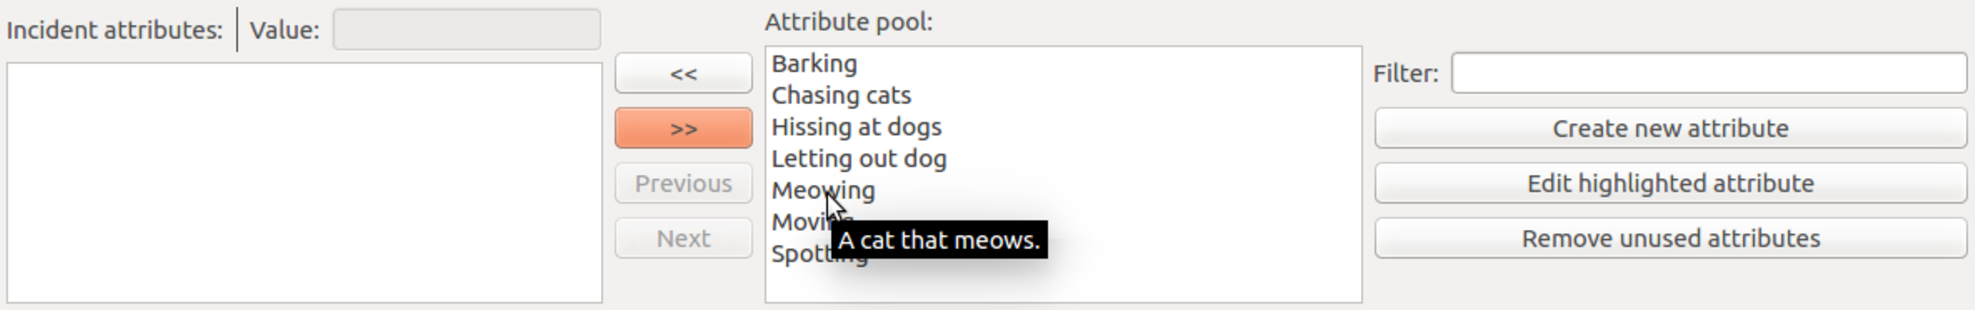
\includegraphics[width=100mm]{Screenshot_9.pdf}
  \label{fig:attributepool}
\end{figure}

\subsection{Filtering attributes}
\label{sec:filteringattributes}

As you are enthusiastically creating new attributes, the \textbf{Attribute pool} will quickly start to fill up, and finding the right attributes to assign to incidents will become a nuisance. That is why I also implemented a filtering option. Filtering works very simple. As soon as you type letters in the dialog, the program will filter out attributes from both the list of \textbf{Incident attributes} and the \textbf{Attribute pool} that do not contain that letter. If you add more letters to the filter, creating a string, then the program will filter out all attributes that do not contain that string (see figure \ref{fig:filteringattributes}). The filter is case sensitive (i.e., 'e' and 'E' are treated as two different cases). 

\begin{figure}[h!]
  \centering
  \caption{Filtering attributes.}
  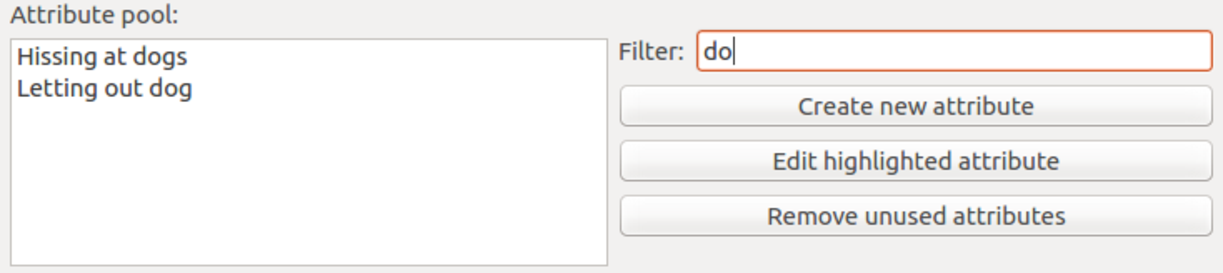
\includegraphics[width=80mm]{Screenshot_10.pdf}
  \label{fig:filteringattributes}
\end{figure}

\subsection{Editing attributes}
\label{sec:editingattributes}

You may occasionally want to edit the label, description, or categories of an attribute that you created earlier. This can be done easily by selecting the attribute in one of the lists (\textbf{Incident attributes} or \textbf{Attribute pool}) and then clicking the \textbf{Edit highlighted attribute} button. Alternatively, you can simply double click any attribute in one of the lists.

This will open the attribute dialog with the details of the existing attribute already shown. Simply edit the details as you like, and save the changes.

\subsection{Removing unused attributes}
\label{sec:removingattributes}

Removing attributes may not be entirely intuitive. I decided not to allow the user to simply click an attribute, and remove it from the \textbf{Attribute pool}. The reason is that the user might have assigned that attribute to another incident, forgotten about this, and thus unintentionally remove the attribute from that incident as well. I therefore assume that one would only ever want to remove attributes that have not been assigned to any incident in the data set. Thus, this is exactly what clicking the \textbf{Remove unused attributes button} will achieve. The program will identify all attributes in the \textbf{Attribute pool} that have not been assigned to some incident in the data set, and then remove these from the program.

Removing unused attributes is an irreversible action, so if you regret removing some attribute, there is no other option than to create it again, from scratch.

Indeed, a drawback of this approach is that it becomes relatively hard to get rid of attributes that you previously assigned to incidents, but do not want to use anymore. Your only option is to find all the incidents to which the attribute has been assigned, unassign the attribute from all of these incidents, and then use the \textbf{Remove unused attributes} option. Indeed, you can make this process less painful by using the following approach:

You could export the data that you have coded so far (see section \ref{sec:exportingdata}), and use the \textbf{"Incident\textunderscore Attributes\textunderscore to\textunderscore Incident\textunderscore Edges.csv"} file to identify the incidents to which the attribute that you want to remove has been assigned. You can then enter the IDs of these incidents in the \textbf{Jump to} dialog to quickly navigate to these incidents, where you can unassign the attribute.


\subsection{Incident attribute categories}
\label{sec:incidentattributecategories}

By now, I have mentioned several times that it is possible to assign categories to attributes (actually, I like to think of this as assigning attributes to categories, but technically there is not really a great difference). In figure \ref{fig:attributedialog} you may have noticed that the attribute dialog itself as a list of assigned \textbf{Categories}, a \textbf{Category pool}, and options to add categories, edit categories, and remove unused categories.

The principles here are the same as with the attributes themselves. Initially, the list of assigned \textbf{Categories} and the \textbf{Category pool} will both be empty. To create a new category, click the \textbf{Add new Category} button. This will open the dialog illustrated in figure \ref{fig:categorydialog}.

\begin{figure}[h!]
  \centering
  \caption{The category dialog.}
  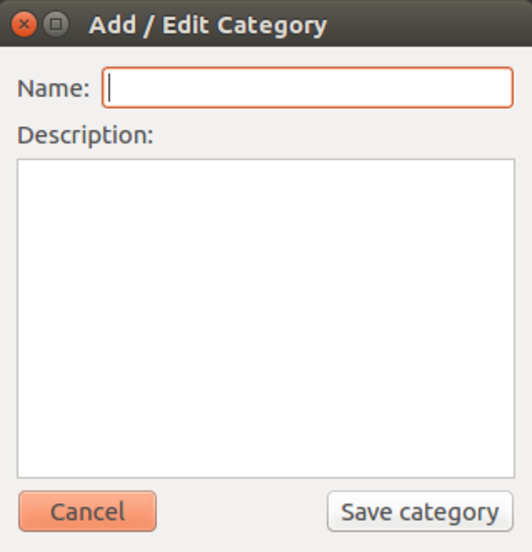
\includegraphics[width=40mm]{Screenshot_11.pdf}
  \label{fig:categorydialog}
\end{figure}

As with attributes, you have to give each category a \emph{unique} name, as well as a description in order to be able to save them. If you change your mind about creating a new category, just click the \textbf{Cancel button}. Otherwise, after assigning a label and offering a description, click the \textbf{Save category} button. To edit a category, select a category in one of the lists (\textbf{Categories} or \textbf{Category pool}) and click \textbf{Edit highlighted category}.

After creating new categories, they will appear in the \textbf{Category pool} in the attribute dialog (see figure \ref{fig:attributedialogwithcategories}). Whenever you are creating a new attribute, or editing an existing attribute, you can assign categories from the \textbf{Category pool} by clicking the assign button (\textbf{\guillemotleft}). To unassign a category, click the unassign button (\textbf{\guillemotright}). In figure \ref{fig:attributedialogwithcategories}, we assigned one category \emph{Dog activities} to the attribute \emph{Barking}. As with attributes, you can hover over the label of any category you created to see the description of that category in a tool tip. 

\begin{figure}[h!]
  \centering
  \caption{Attribute with assigned category.}
  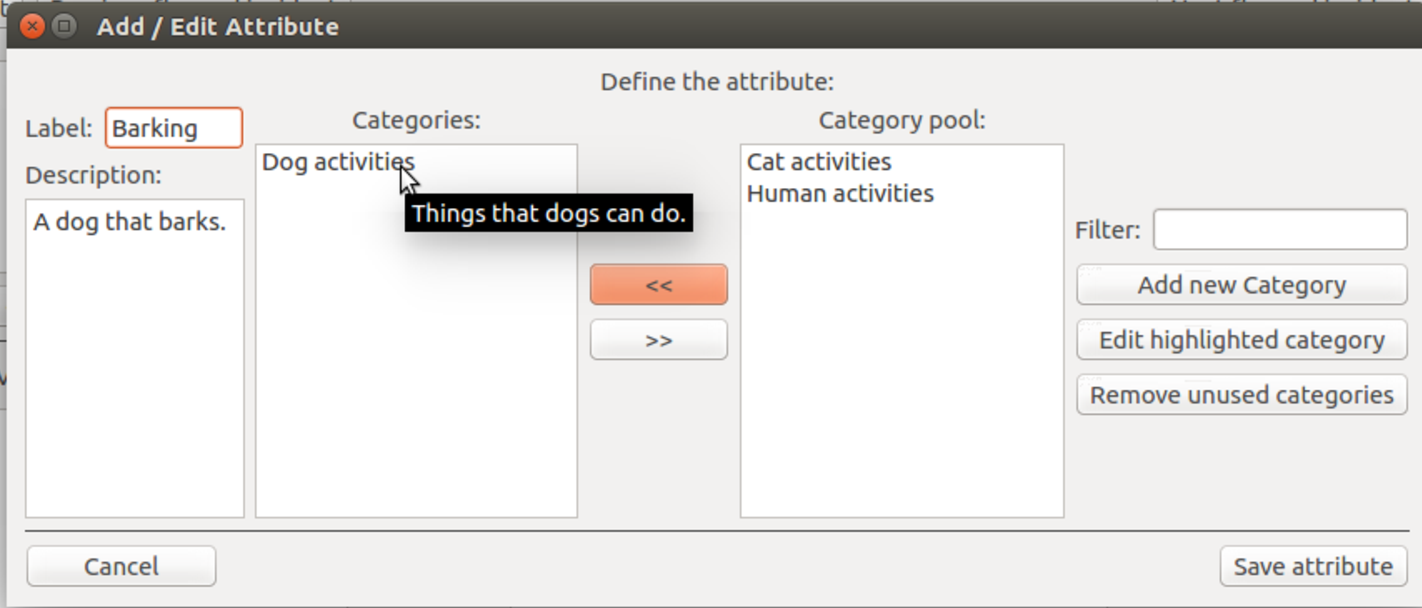
\includegraphics[width=100mm]{Screenshot_12.pdf}
  \label{fig:attributedialogwithcategories}
\end{figure}

Removing categories also works similar to removing attributes, which means that you can only remove all categories that are not currently in use by clicking the \textbf{Removed unused categories} button. If you want to remove a category that you have already assigned to various attributes, you might want to consider the following approach:

Export the data that you have coded so far (see section \ref{sec:exportingdata}), and check the file \textbf{``Entity\textunderscore Attributes\textunderscore to\textunderscore Categories\textunderscore Edges.csv''} to identify the attributes to which the category has been assigned. Then, in the main dialog of the program, use the filter to quickly find these attributes (they could appear in the list of \textbf{Incident attributes} or the \textbf{Attribute pool}, depending on whether they were assigned or not). Then edit these attributes (e.g., double click their label) and unassign the category you intend to remove from them. After unassigning the category from all attributes in this way, remove the category by clicking the \textbf{Remove unused categories} button.

\subsection{Assigning and unassigning attributes}
\label{sec:assigningunassigningattributes}

Once you have created attributes, you can start assigning them to incidents. Assigning an attribute to an incident can be done by selecting the attribute in the \textbf{Attribute pool}, and then clicking the assign button (\textbf{\guillemotleft}). The attribute will move from the \textbf{Attribute pool} to the list of \textbf{Incident attributes}, and the attribute is now associated with this incident. In figure \ref{fig:assignedattributes} we have assigned one attributes to the current incident, based on the description of the incident available to us.

\begin{figure}[h!]
  \centering
  \caption{Attributes assigned to incident.}
  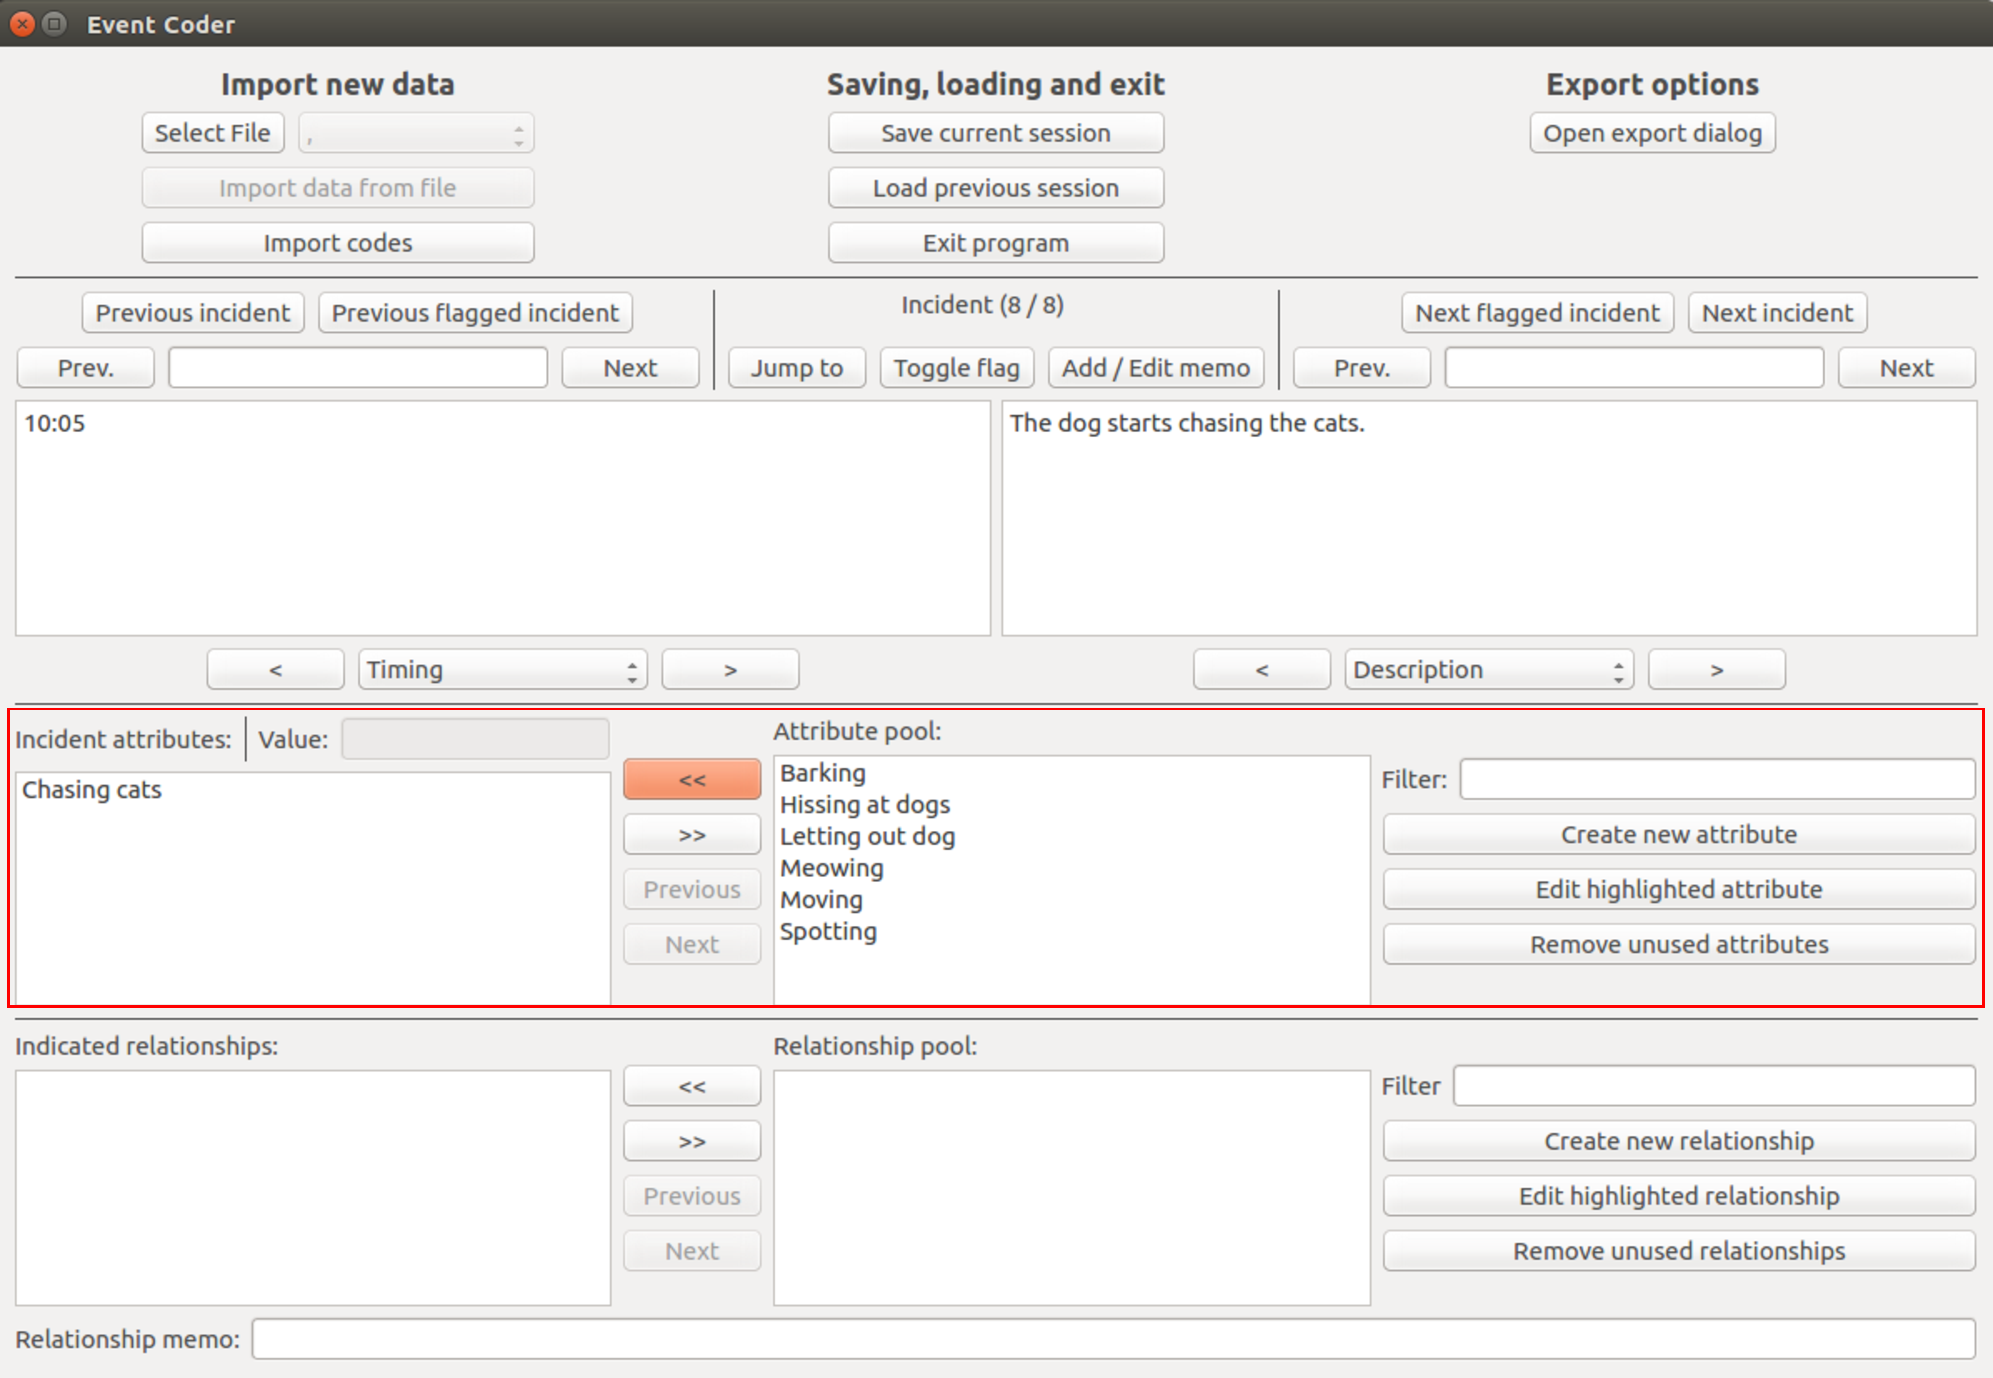
\includegraphics[width=100mm]{Screenshot_13.pdf}
  \label{fig:assignedattributes}
\end{figure}

In this case, we have also done something else: we have added a value to the attribute, by clicking on the assigned variable, and then typing ``5 cats'' in the value field, which is located above the list of \textbf{Incident attributes}, to indicate that the dog is chasing 5 cats in total.

If we decide that this value is not important after all, we could just select the attribute again, and delete the value that we entered.

And with this we have covered everything important that there is to know about the attribute module of the program!

\section{The relationship module}
\label{sec:relationshipmodule}

The other module that can be used for coding purposes is the relationship module. This module can be found at the bottom of the main dialog of the program (see figure \ref{fig:relationshipmodule}). Its primary purpose is to identify relationships between entities that are indicated by the incidents under consideration. 
\begin{figure}[h!]
  \centering
  \caption{The relationship module.}
  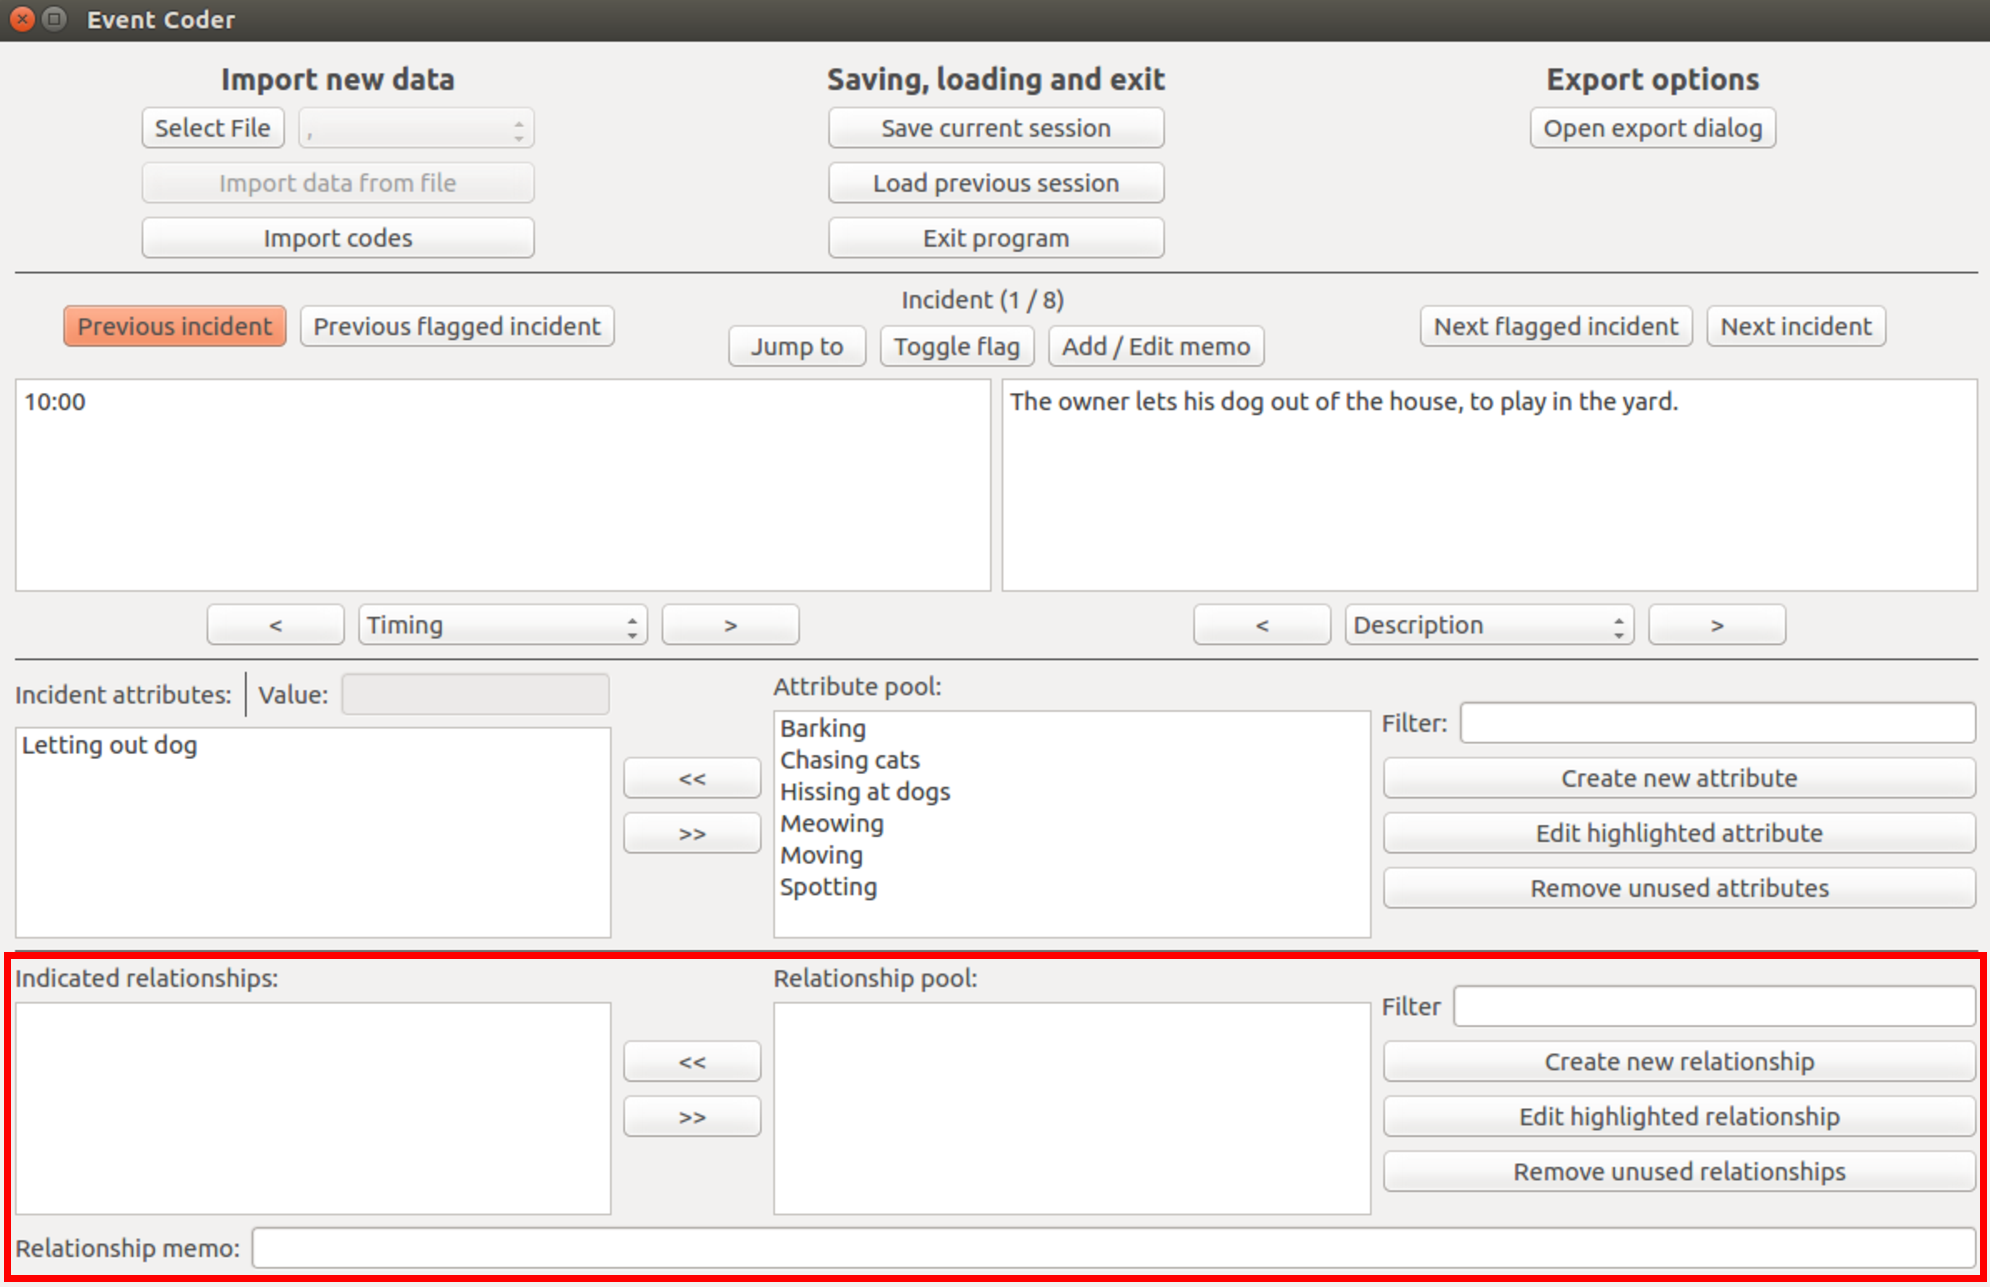
\includegraphics[width=100mm]{Screenshot_14.pdf}
  \label{fig:relationshipmodule}
\end{figure}

For example, say that we have a set of incidents that describe how a dog encounters a cat in his yard, which it then proceeds to chase out of the yard. There are several relationships that we could possibly refer from this (although for most we would perhaps need a bit more context). For example, we could infer that the dog considers the yard as his territory (\(Yard-[is\  territory\ of]\rightarrow Dog\)), we could infer that the dog hates the cat (\(Dog-[hates]\rightarrow Cat\)), and we could infer that the cat is afraid of the dog (\(Cat-[is\ afraid\ of]\rightarrow Dog\)). These are examples of relationships that could be identified with the relationship module of the program, and the idea is that the incidents are used as evidence for the existence of the relationships.

\subsection{Creating new relationships - part 1}
\label{sec:creatingnewrelationships1}

If you have not yet created relationships, the list of \textbf{Indicated relationships} and the \textbf{Relationship pool} will both be empty. If you want to assign relationships to the current incident (i.e., identify a relationship that is indicated by the incident), you will first need to create one. This takes a number of steps. The first step is to click the \textbf{Create new relationship} button. This will open the relationship dialog (see figure \ref{fig:relationshipdialog}).

\begin{figure}[h!]
  \centering
  \caption{The relationship dialog.}
  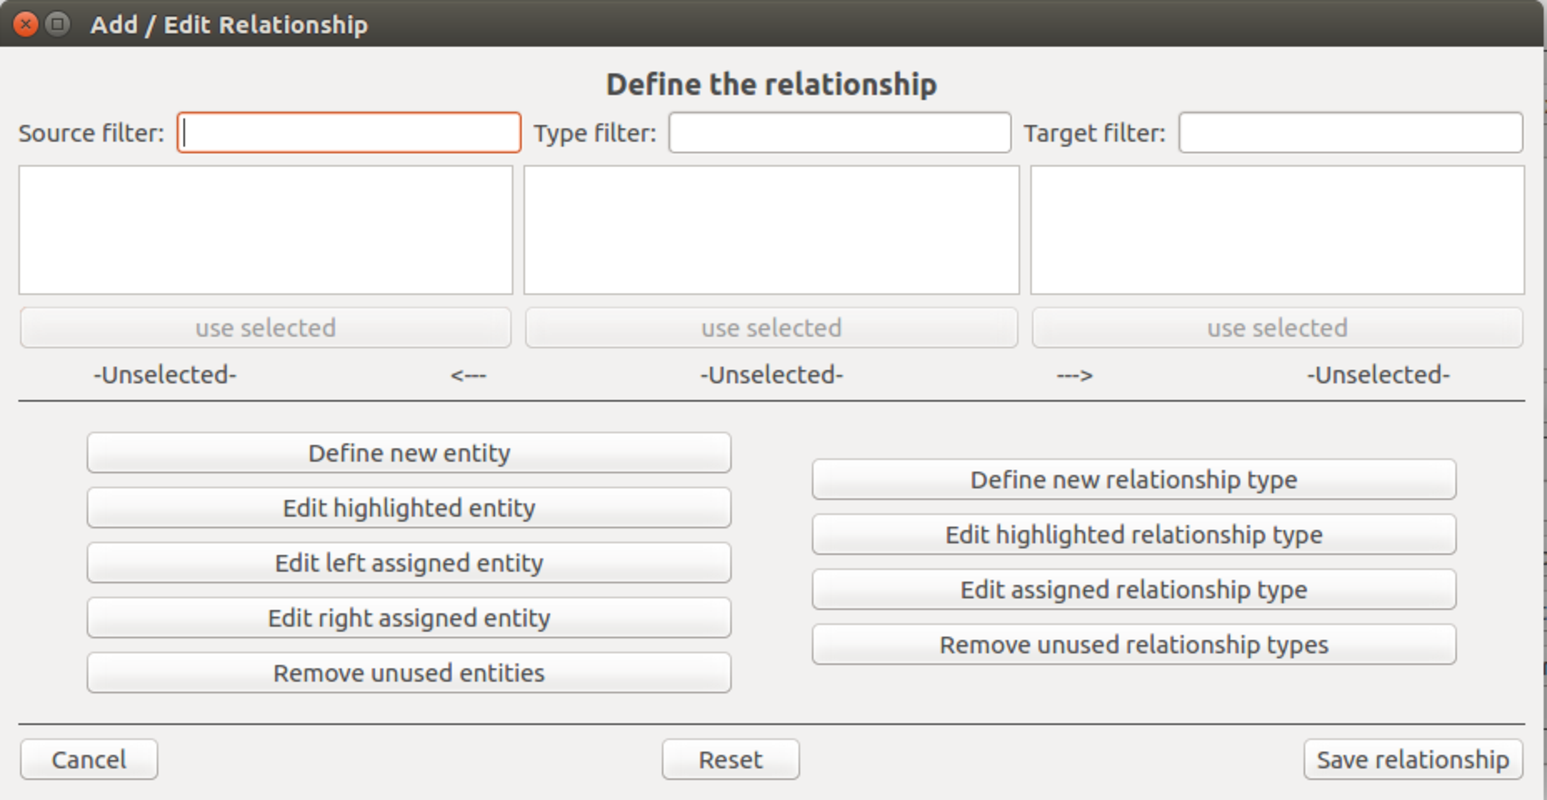
\includegraphics[width=100mm]{Screenshot_15.pdf}
  \label{fig:relationshipdialog}
\end{figure}

This dialog indeed looks quite different from the attribute dialog. In this case, we have three fields, which can be used to select (from left to right) the \textbf{source node} of the relationships, the \textbf{type} of the relationship, and the \textbf{target node} of the relationship. The \textbf{source node} and \textbf{target node} are always entities. \textbf{Relationship types} have a label, a description, and also a direction, which can be \textbf{directed} or \textbf{undirected}. In order to be able to create relationships, you first need to create entities and relationship types. We have to discuss this in detail before we can finish our discussion on creating relationships.

\subsection{Entities}
\label{sec:entities}

A new entity can be create by clicking the \textbf{Define new entity} button. This will open a new dialog (see figure \ref{fig:entitydialog}).

\begin{figure}[h!]
  \centering
  \caption{The entity dialog.}
  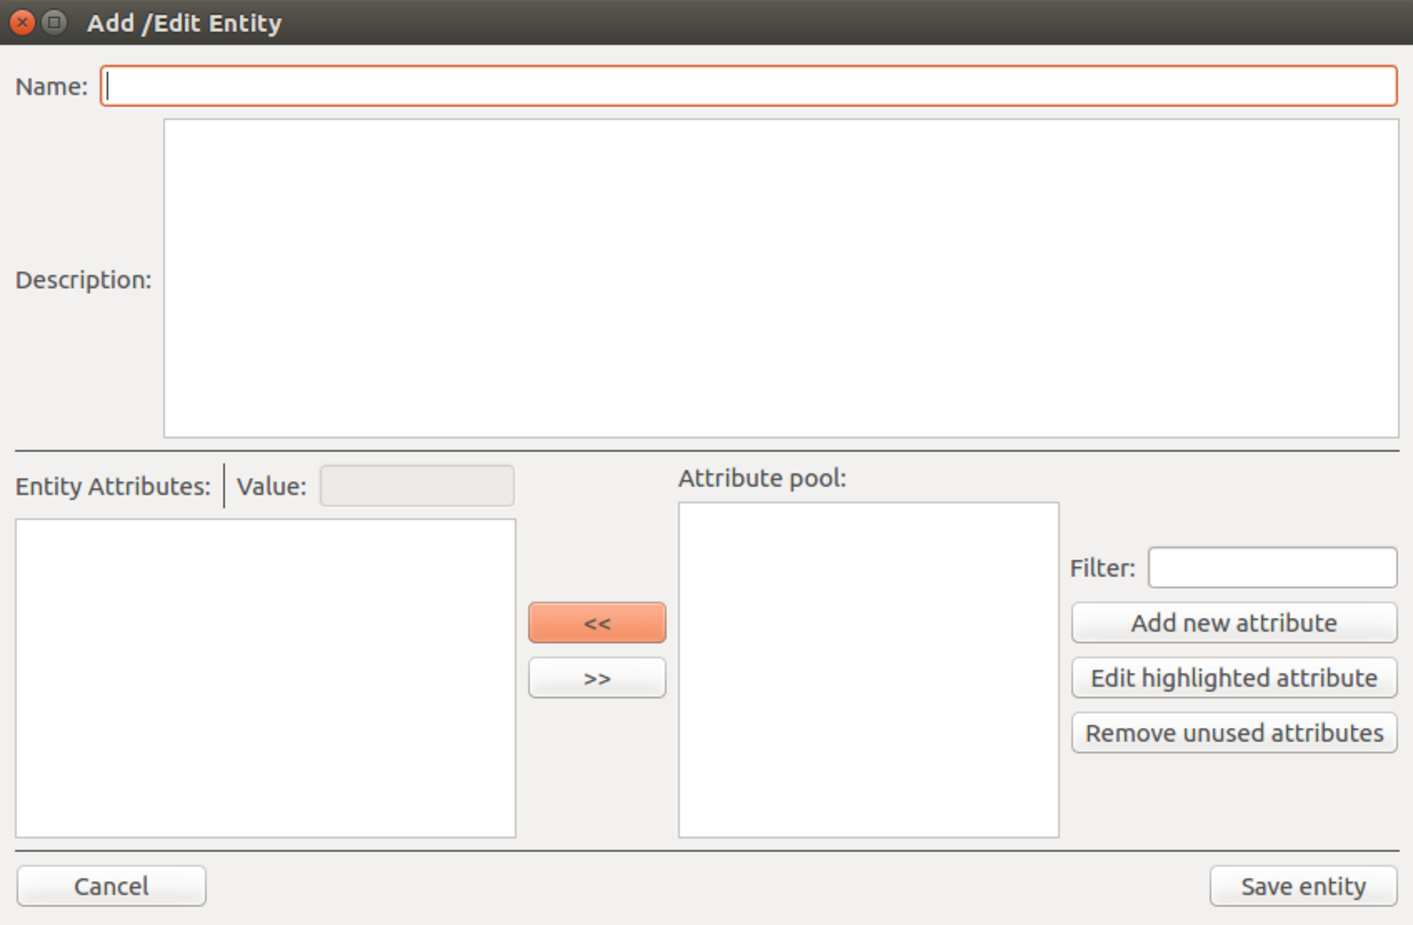
\includegraphics[width=100mm]{Screenshot_16.pdf}
  \label{fig:entitydialog}
\end{figure}

Similar to attributes, entities always require (1) a \emph{unique} name, and (2) a description. The name will be used throughout the program to refer to the entity. Optionally, you can also assign attributes to entities. \textbf{Assigning attributes to entities works the exact same as assigning attributes to incidents. I therefore do not explain this procedure here, but refer you to section \ref{sec:attributemodule}}. The program does, of course, make a distinction between attributes (and their categories) associated with incidents, and attributes (and their categories) associated with entities. 

Once you have created a new entity, it will appear in the \textbf{source node} selection field, and the \textbf{target node} selection field (see figure \ref{fig:relationshipdialog2}).

As with the attributes and categories, editing entities in these lists can be done by selecting them, and clicking the \textbf{Edit highlighted entity} button. This will open an entity dialog with the corresponding information already included. 

As with attributes and categories, it is only possible to remove entities that are not currently in use, which in this case means that you can only remove entities that are not participating in one of the relationships that have been defined (whether that relationship itself has been used or not).

To remove unused entities, click the \textbf{Remove unused entities} button. Before doing this, you might first want to remove unused relationships (see section \ref{sec:removingrelationships}). This should also free up any entities that were assigned to unused relationships.

\subsection{Relationship types}
\label{sec:relationshiptypes}

To create a new relationship type, click the \textbf{Define new relationship type} button. This will open the relationship type dialog (see figure \ref{fig:relationshiptypedialog}). 

\begin{figure}[h!]
  \centering
  \caption{Relationship type dialog.}
  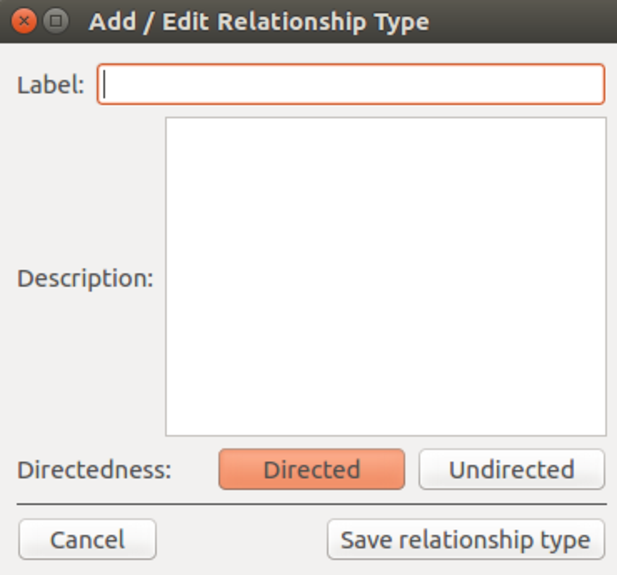
\includegraphics[width=50mm]{Screenshot_17.pdf}
  \label{fig:relationshiptypedialog}
\end{figure}

As with attributes, entities and categories, new relationship types can only be saved if you have assigned both a label and a description to them. In the case of relationship types you also need to indicate the direction of the relationship, which is set to \textbf{Directed} by default. In a direction relationship, the relationship is always directed from the \textbf{source node} to the \textbf{target node} (e.g., \(source-[likes]\rightarrow target\)). In an \textbf{undirected} relationship, there is no direction, and the \textbf{source node} and the \textbf{target node} are interchangeable (e.g., \(source-[talks with]\rightarrow target\)). 

Once you have created a new relationship type, it will appear in the \textbf{Relationship type} selection field (see figure \ref{fig:relationshipdialog2}).

As with the attributes, categories, and entities, editing relationship types in these lists can be done by selecting them, and clicking the \textbf{Edit highlighted relationship type} button. This will open a relationship type dialog with the corresponding information already included. 

As with attributes, categories an entities, it is only possible to remove relationship types that are not currently in use, which in this case means that you can only remove relationship types that are not participating in one of the relationships that have been defined (whether that relationship itself has been used or not).

To remove unused relationship types, click the \textbf{Remove unused relationship types} button. Before doing this, you might first want to remove unused relationships (see section \ref{sec:removingrelationships}). This should also free up any relationship types that were assigned to unused relationships.

\subsection{Creating new relationships - part 2}
\label{sec:creatingnewrelationships2}

\begin{figure}[h!]
  \centering
  \caption{The relationship dialog with entities and relationship types available for selection.}
  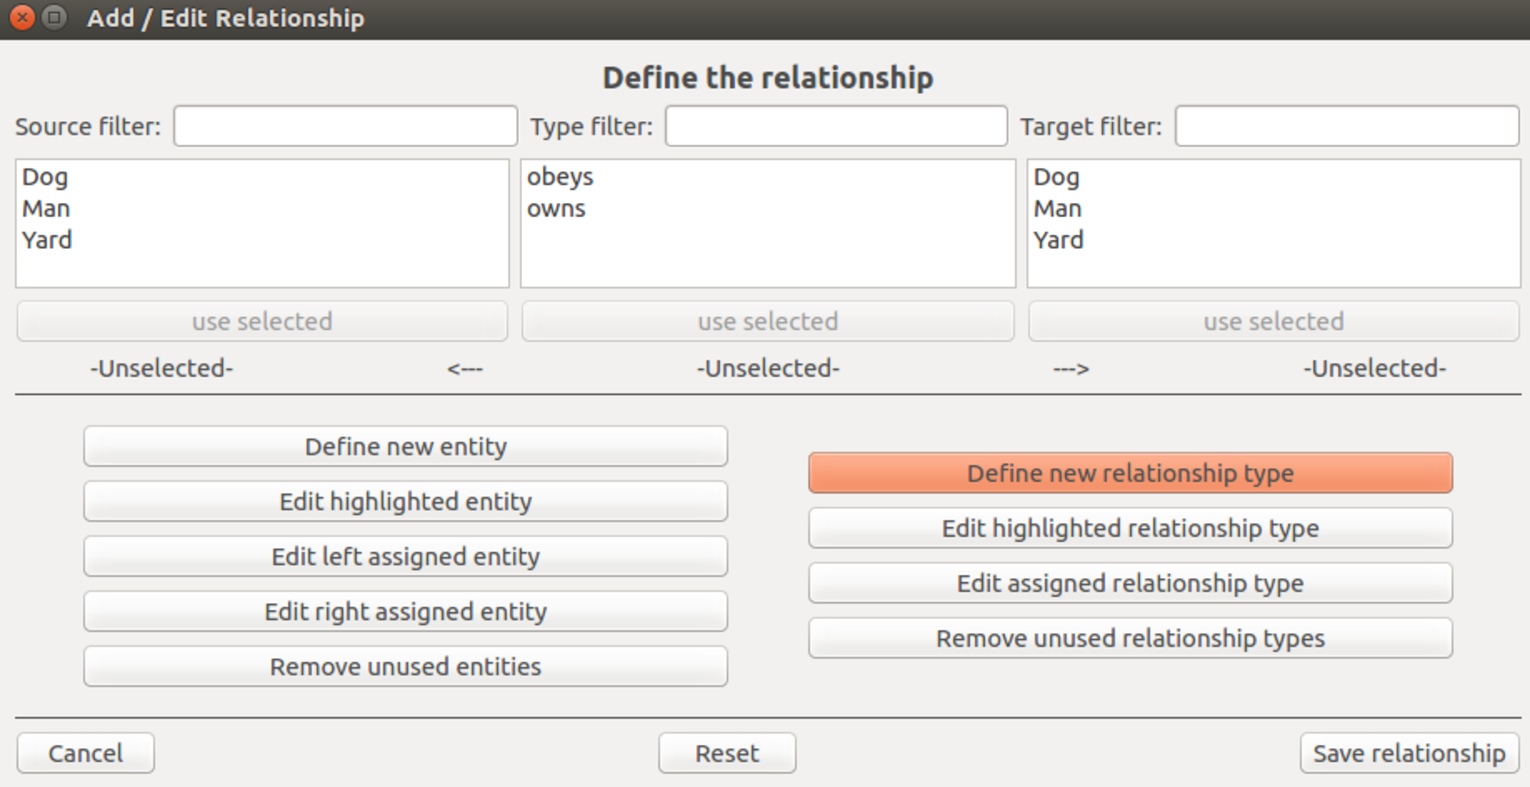
\includegraphics[width=100mm]{Screenshot_18.pdf}
  \label{fig:relationshipdialog2}
\end{figure}

\subsection{Editing relationships}
\label{sec:editingrelationships}



\subsection{Removing relationships}
\label{sec:removingrelationships}


\chapter{What is next?}
\label{chap:whatisnext}

So, you have coded a data set (see chapter \ref{chap:usingtheprogram2}), and you have exported your coded data (see section \ref{sec:exportingdata}), resulting in a bunch of files in the \textbf{``export/''} folder. What can we actually do with those files now? 


\chapter{Contact details}
\label{chap:contactdetails}





\end{document}